\documentclass[openany,11pt,vi,oneside]{mitthesis}
\usepackage{lgrind}
\usepackage{calc}
\usepackage{cmap}
\usepackage{mathtools}
\usepackage{amssymb}
\usepackage{bm}
\usepackage{enumitem}
\usepackage{scrextend}
\usepackage{lscape}
\usepackage{geometry}
\usepackage{multicol}
\usepackage{multirow}
\usepackage{xcolor}
\usepackage{float}
\usepackage{lscape}
\usepackage{tabu}
\usepackage{graphicx}
\usepackage{subcaption}
\usepackage{nameref}
%\usepackage{xifthen}
\usepackage{tikz}
\usepackage{matlab-prettifier}
\usepackage{listings}
%\usepackage{acronym}
\usepackage{hyperref}
\usepackage[hang]{footmisc}
\usetikzlibrary{shapes,arrows.meta,calc}
\usepackage[backend=biber,
			style=numeric, maxcitenames=1, sorting=none, url=false, isbn=false, doi=true, eprint=false]{biblatex}
\hypersetup{colorlinks,citecolor={purple},linkcolor={blue}}
%%%%%%%%%%%%%%%%%%%%%%%%%%%%%%%%%%%%%%%%%%%%%%%%%%%%%%%%%%%%%%%%%%%%%%%%%%%%%%%%%%%%%%%%%%%%%%%%%%%%
% resources
%\include{src}
%\include{matrices}
\addbibresource{C:/Users/Jesse/Documents/tex/src/tex/latex/library.bib}
\graphicspath{{figs/}{figs/tikz/}{figs/tikz/algorithm/}}
\newcommand{\matlabdir}{C:/Users/Jesse/Documents/m/Research/wmlseg/workspace/}
% layout
\geometry{margin=2cm}
\setlength{\parindent}{0pt}
\setlength{\parskip}{8pt}
\setlength{\skip\footins}{24pt}
\setlength{\footnotemargin}{0.8em}
%%%%%%%%%%%%%%%%%%%%%%%%%%%%%%%%%%%%%%%%%%%%%%%%%%%%%%%%%%%%%%%%%%%%%%%%%%%%%%%%%%%%%%%%%%%%%%%%%%%%
% math shorthands
\renewcommand{\Re}{\mathbb{R}}
\newcommand{\x}{\mathbf{x}}
\newcommand{\gm}{\textsc{gm}}
\newcommand{\wm}{\textsc{wm}}
\newcommand{\csf}{\textsc{csf}}
\newcommand{\les}{\textsc{les}}
\newcommand{\mrf}{\textsc{mrf}}
\newcommand{\lr}{\textsc{lr}}
\newcommand{\K}{\textsc{k}}
\newcommand{\N}{\textsc{n}}
\renewcommand{\d}{\partial}
\renewcommand{\b}{\beta}
\newcommand{\bb}{\bm{\beta}}
\newcommand{\by}{\bm{y}}
\renewcommand{\L}{\mathcal{L}}
\renewcommand{\N}{\mathcal{N}}
\newcommand{\J}{\mathcal{J}}
\newcommand{\X}{\mathcal{X}}
\newcommand{\Y}{\mathcal{Y}}
\newcommand{\C}{\mathcal{C}}
\newcommand{\bX}{\bm{\mathcal{X}}}
\newcommand{\bY}{\bm{\mathcal{Y}}}
\newcommand{\bC}{\bm{\mathcal{C}}}
\newcommand{\abs}[1]{\left|#1\right|}
\newcommand{\norm}[1]{\left|\left|#1\right|\right|}
% colors
\definecolor{c01}{rgb}{1.00 0.00 0.00}
\definecolor{c02}{rgb}{1.00 0.38 0.00}
\definecolor{c03}{rgb}{1.00 0.75 0.00}
\definecolor{c04}{rgb}{0.13 0.80 0.00}
\definecolor{c05}{rgb}{0.00 0.80 0.80}
\definecolor{c06}{rgb}{0.00 0.50 1.00}
\definecolor{c07}{rgb}{0.00 0.20 1.00}
\definecolor{c08}{rgb}{0.50 0.00 1.00}
\definecolor{c09}{rgb}{1.00 0.00 1.00}
\definecolor{c10}{rgb}{0.50 0.50 0.50}
\definecolor{gry}{rgb}{0.50 0.50 0.50}
% little text items
\renewcommand{\ss}[1]{\textsuperscript{#1}}
\newcommand{\hreftt}[1]{\href{#1}{\texttt{#1}}}
\newcommand{\et}{\thinspace}
\newcommand{\en}{\enspace}
% sizing
\newcommand{\plotwidth}{0.48\textwidth}
% appendix
\newcommand{\matlabsty}{\color{black}\ttfamily\footnotesize}
%\lstMakeShortInline[style=Matlab-editor,basicstyle=\matlabsty]@
\lstnewenvironment{matlab}{\lstset{style=Matlab-editor,basicstyle=\matlabsty}}{}
\newcommand{\includecode}[1]{\subsubsection{\ttfamily{#1}}
  \begin{singlespace}\lstinputlisting[style=Matlab-editor,basicstyle=\linespread{0}\matlabsty]{\matlabdir#1}\end{singlespace}}
%%%%%%%%%%%%%%%%%%%%%%%%%%%%%%%%%%%%%%%%%%%%%%%%%%%%%%%%%%%%%%%%%%%%%%%%%%%%%%%%%%%%%%%%%%%%%%%%%%%%
\begin{document}
% \title{Voxel-Wise Image Analysis\\for White Matter Hyperintensity Segmentation}
\author{Jesse Knight}
\department{School of Engineering}
\degree{Master of Applied Science in Engineering Systems and Computing}
\degreemonth{}
\degreeyear{2017}
\thesisdate{2017-12-18}
\copyrightnoticetext{}
\maketitle
\cleardoublepage{}
\pagenumbering{Roman}
\setcounter{page}{1}
\begin{abstractpage}
  White matter hyperintensities (WMH) are regions of increased pixel intensity
in T2-weighted MRI which are correlated with several neurodegenerative diseases.
Human segmentation of WMH is time consuming and inconsistent,
motivating automation of WMH segmentation.
\par
While many algorithms for this task have previously been proposed,
few have been validated on MRI from different sources,
despite the sensitivity of most algorithms to source-specific image features.
\par
This thesis presents a segmentation algorithm called
``Voxel-Wise Logistic Regression'' (VLR),
which provides both good interpretability and segmentation performance.
VLR uses FLAIR MRI to estimate the WMH class probability image using
spatially varying logistic parameters $\bm{\beta}(x)$.
These ``parameter images'' also concisely summarize the model class discrimination.
\par
Additionally, a validation framework called
``Leave-One-Source-Out Cross Validation'' (LOSO-CV) is introduced,
which provides more realistic estimation of model performance
on ``never-before-seen'' MRI sources.
Segmentation performance of the VLR model under LOSO-CV
is presented using 96 open-source images from 7 MRI sources.

\end{abstractpage}
\cleardoublepage{}
\begin{titlepage}
  \begin{large}
    This masters thesis has been examined by \\ a Committee of the School of Engineering as follows:
    \signature{Hadis Karimipour}{Chair, Thesis Examination Committee \\
      Assistant Professor\\
      University of Guelph}
    \signature{April Khademi}{Thesis Co-Supervisor \\
      Assistant Professor\\
      Ryerson University}
    \signature{Graham Taylor}{Thesis Co-Supervisor \\
      Associate Professor\\
      University of Guelph}
    \signature{Medhat Moussa}{Member, Thesis Examination Committee \\
      Professor\\
      University of Guelph}
  \end{large}
\end{titlepage}
\section*{Acknowledgments}
I owe thanks to \dots
\\Jeremy, Danny, and Carly, for our cherished polemic forums;
\\Daniel, for sharing with me passions, pizza, and almost projects;
\\Thor, Colin, Terrance, and Dylan for our `deep' conversations;
\\Brayden, Aaron, and Carson, for board games and Jamaican bacon;
\\Erika, Denise, Emily, and Zyra, for bunting, crosswords, and Harambe;
\\My parents and Ali, for all your love and support;
\\and
\\My supervisors, for sharing with me your time, expertise, and so many opportunities.
\vfill
\begin{singlespace}
  \hspace*{4.0cm}\textit{If you want the truth to stand clear before you,}\\
  \hspace*{4.5cm}\textit{never be for or against.}                        \\
  \hspace*{4.0cm}\textit{The struggle between `for' and `against'}        \\
  \hspace*{4.5cm}\textit{is the mind's worst disease.}                    \\[0.5em]
  \hspace*{9.0cm}\normalfont --- Sent-ts'an c. 700 C.E.
\end{singlespace}

% \begin{abstract}White matter hyperintensities (WMH) are regions of increased pixel intensity
in T2-weighted MRI which are correlated with several neurodegenerative diseases.
Human segmentation of WMH is time consuming and inconsistent,
motivating automation of WMH segmentation.
\par
While many algorithms for this task have previously been proposed,
few have been validated on MRI from different sources,
despite the sensitivity of most algorithms to source-specific image features.
\par
This thesis presents a segmentation algorithm called
``Voxel-Wise Logistic Regression'' (VLR),
which provides both good interpretability and segmentation performance.
VLR uses FLAIR MRI to estimate the WMH class probability image using
spatially varying logistic parameters $\bm{\beta}(x)$.
These ``parameter images'' also concisely summarize the model class discrimination.
\par
Additionally, a validation framework called
``Leave-One-Source-Out Cross Validation'' (LOSO-CV) is introduced,
which provides more realistic estimation of model performance
on ``never-before-seen'' MRI sources.
Segmentation performance of the VLR model under LOSO-CV
is presented using 96 open-source images from 7 MRI sources.
\end{abstract}
	%\pagenumbering{Roman}
\begin{singlespacing}
\tableofcontents
\newpage
\listoffigures
\newpage
\listoftables
\newpage
\subsection*{Abbreviations}
\begin{table}[H]
  \begin{tabular}{ll}
  	\hline
  	GM      & Grey matter                          \\
  	WM      & White matter                         \\
  	CSF     & Cerebrospinal fluid                  \\
  	PD      & Proton density                       \\
  	FLAIR   & Fluid attenuation inversion recovery \\
  	WML     & White matter lesion                  \\
  	WMH     & White matter hyperintensity          \\
  	DAWM    & Dirty appearing WM                   \\
  	MS      & Multiple Sclerosis                   \\
  	AD      & Alzheimer's Disease                  \\
  	PVE     & Partial volume effect                \\
  	VLR     & Voxel-Wise Logistic Regression       \\
  	MLE     & Maximum likelihood estimation        \\
  	MAP     & Maximum a posteriori                 \\
  	SI      & Similarity index                     \\
  	ICC     & Interclass Correlation Coefficient   \\
  	LL      & Lesion load                          \\
  	CV      & Cross validation                     \\
  	LOO-CV  & Leave-one-out CV                     \\
  	KF-CV   & K-fold CV                            \\
  	LOSO-CV & Leave-one-source-out                 \\
  	SVM     & Support vector machine               \\
  	K-NN    & K-nearest neighbours                 \\
  	MRF     & Markov random field                  \\
  	FPR     & False positive reduction             \\ \hline
  \end{tabular}
\end{table}
\clearpage
\subsection*{Notation}
\begin{table}[H]
  \begin{tabular}{lll}
  	\hline
  	\multicolumn{3}{l}{Variables}                                                                                            \\ \hline
  	$y$                   & feature                                                                    & $\in\Re$            \\
  	$\tilde{y}$           & standardized feature                                                       & $\in\Re$            \\
  	$c$                   & true class                                                                 & $\in\{0,1\}$        \\
  	$\hat{c}$             & estimated class                                                            & $\in[0,1]$          \\
  	$\beta$               & logistic model feature weight                                              & $\in\Re$            \\
  	$\gamma$              & synthetic feature                                                          & $\in\Re$            \\
  	$\rho$                & prior probability                                                          & $\in[0,1]$          \\ \hline
  	\multicolumn{3}{l}{Indexing -- e.g. arbitrary variable $a$}                                                              \\ \hline
  	$k$                   & feature index                                                              & $\in \{1,\dots,K\}$ \\
  	$n$                   & subject index                                                              & $\in \{1,\dots,N\}$ \\
  	$t$                   & iteration index                                                            & $\in \{1,\dots,X\}$ \\
  	$x$                   & spatial location                                                           & $= [\xxx]$          \\
  	${a_n^k}^{(t)}(x)$    & $k$\ss{th} feature; $n$\ss{th} subject; $t$\ss{th} iteration; location $x$ &                     \\ \hline
  	\multicolumn{3}{l}{Images \& sets -- e.g. arbitrary variable $a$}                                                        \\ \hline
  	$a$                   & one voxel, one feature, one subject                                        &                     \\
  	$\bm{a}$              & one voxel, all features, one subject                                       &                     \\
  	$\mathrm{A}(x)$       & image in native space                                                      &                     \\
  	$A(x)$                & image in standard space (MNI)                                              &                     \\
  	$\bm{A}(x)$           & image set: all features, one subject                                       &                     \\
  	$\mathcal{A}(x)$      & image set: one feature, all subjects                                       &                     \\
  	$\bm{\mathcal{A}}(x)$ & image superset: all features, all subjects                                 &                     \\
  	$\x{A}$               & full dataset: all features, subjects, voxels                               &                     \\ \hline
  \end{tabular}
\end{table}
\end{singlespacing}
\clearpage
\pagenumbering{arabic}
\setcounter{page}{1}

  %%%%%%%%%%%%%%%%%%%%%%%%%%%%%%%%%%%%%%%%%%%%%%%%%%%%%%%%%%%%%%%%%%%%%%%%%%%%%%%%%%%%%%%%%%%%%%%%%%%%
% ==================================================================================================
% --------------------------------------------------------------------------------------------------
\chapter{Introduction}
Digitization of medical imaging has facilitated innumerable advances in disease understanding and treatment. From multi-modal image fusion to image guided therapy, software tools now underpin research and clinical workflows in almost every domain of medical imaging.
\par
This work concerns an unsolved segmentation problem in 3D brain magnetic resonance imaging (MRI), in which the objective is to automatically predict the class, or label, of every voxel (``volume pixel'') in the image. The objects of interest are white matter hyperintensities (WMH), non-cancerous brain lesions which are correlated with several neurodegenerative diseases. This chapter presents the motivation for automated WMH segmentation, gives a problem definition, and explores the previously proposed solutions.
%%%%%%%%%%%%%%%%%%%%%%%%%%%%%%%%%%%%%%%%%%%%%%%%%%%%%%%%%%%%%%%%%%%%%%%%%%%%%%%%%%%%%%%%%%%%%%%%%%%%
\section{Motivation}
The brain is composed of three major classes of tissue: grey matter (GM), white matter (GM), and cerebrospinal fluid (CSF). Grey matter constitutes the peripheral surface of the brain -- the cortex, approximately 5mm thick -- as well as some deeper structures called the basal ganglia. It contains neuronal cell bodies, and performs the bulk of neural processing. The white matter is composed primarily of myelinated axons, and functions to relay information between different GM structures in the brain. The brain is surrounded by CSF, which provides mechanical and immunological defence. It is produced by the choroid plexuses in the ventricles of the brain -- a series of 4 connected cavities.
\par
...
% ==================================================================================================
\subsection{White Matter Disease}
``Normal'' ageing of the brain is characterized by a variety of physical and cognitive changes. Memory, synaptic plasticity, and brain volume decline, with observable effects on cognitive function \cite{Peters2006,Good2002}. Brain ageing is also expedited in many patients by neurodegenerative diseases targeting the white matter, including Alzheimer's disease (AD), cerebrovascular disease, and in rare cases Multiple Sclerosis (MS). While the etiologies of these diseases are not yet fully understood, there is considerable evidence to suggest that the they are intertwined \cite{Debette2010,Conklin2014,Heppner2015,Snyder2015}.
\par
Cerebrovascular disease describes changes to blood vessels in the brain which increase the risk of ischemic injury -- a reduction in blood flow due to vessel occlusion or hemorrhage. Ischemic injuries include major events (stroke) \cite{VanderWorp2007}, transient ischemic attacks \cite{Albers2002}, and chronic hypoperfusion due to small vessel disease \cite{Pantoni2010}. In all such events, neuronal death occurs from insufficient nutrient supply \cite{VanderWorp2007}. Strokes involving major cerebral arteries can be fatal, and post-event quality of life in survivors is highly variable \cite{Prabhakaran2015}. In the less dramatic courses, clinically quiet disease progression can lead to personality changes, memory loss, and reduced cognitive ability; such changes are termed vascular dementia \cite{Roman1993}.
\par
Alzheimer's Disease is another subclass of dementia with similar symptoms; in fact it is the most common type, affecting about 6\% of the population over age 65 \cite{Burns2009}. The cause of Alzheimer's disease is hotly debated. Two 30-year-old theories linking the disease to the build up of amyloid $\beta$ protein and misfolded protein $\tau$ have been widely supported by correlational studies \cite{Masters1985,Hardy2002,Lee2011}, but have lacked clear mechanisms of injury until recently. It is now thought that amyloid $\beta$ oligomers interfere with neuronal mitochondria and synapse function, leading to cell death \cite{Kim2013,Tu2014}, while aberrant $\tau$ proteins disrupt microtubules necessary for intraneuronal transport \cite{Lee2011}. During the search for these mechanisms, competing theories implicating vascular injury \cite{Snyder2015}, immune response \cite{Heppner2015}, and blood brain barrier disruption \cite{Bell2009} have emerged, painting the picture of a more complex disease.
\par
The pathophysiology of multiple sclerosis is similarly unclear, though genetics are a necessary factor, and it is known that symptoms arise from erosion of myelin -- a fatty insulating layer surrounding axons which is critical for normal neuron firing \cite{Trapp2008}. Several theories hypothesize either that this damage is driven by autoimmune attack, followed by neuronal dysfunction and death, or that neurodegenerative changes stimulate recruitment of immune cells as part of the usual response to injury \cite{Lucchinetti2000,Trapp2008}. Recent evidence favours the former mechanism, particularly with inflammatory injury as the initiating event \cite{Ciccarelli2014,Mahad2015}.
%A helpful visualization of MS lesion progression over one year is available here\footnote{\hreftt{http://www.msdiscovery.org/sites/default/files/MGrid\_crop4\_full\_0.gif}}.
\par
Connecting all these diseases are white matter lesions (WML, \textsc{aka} Leukoariosis), which represent the macroscopic changes to brain tissue in regions of white matter damage \cite{Debette2010,Bakshi2005,Wardlaw2015}. WML are very common in elderly populations, and a small volume of lesion does not necessarily implicate one of the above diseases; in one study of 1077 subjects aged 60-90, 95\% had at least one WML \cite{DeLeeuw2001}. WML appear as bright tissue regions in T2-weighted MRI due to some combination of inflammatory injury and degradation of tissue structure \cite{Bakshi2005,Wardlaw2015}; in this imaging context, they are often called white matter hyperintensities (WMH). Lesions are often focal, as opposed to diffuse, but there is evidence to suggest that surrounding regions of moderate hyperintensity, sometimes called ``dirty appearing white matter (DAWM)'', are also related to the diseases \cite{Ge2003}. As biomarkers of the most common WM diseases -- conditions with unsolved etiologies and inadequate treatments -- WML are of special interest to many brain researchers. MR imaging of WMH is used for both research and patient management; before discussing how, the principals of MRI are first introduced.
% ==================================================================================================
\subsection{Magnetic Resonance Imaging}
Magnetic resonance imaging (MRI) provides superior and flexible brain tissue contrast versus computed tomography (CT) imaging, and is the primary modality for imaging white matter disease. Whereas CT measures tissue density via attenuation of transmitted X-rays, which does not vary significantly among brain tissues, MRI measures a mutable combination of 3 tissue characteristics: the proton density (PD)\footnote{MRI can be used to image any nucleus with a net nuclear dipole, but proton (hydrogen) imaging is most common since hydrogen is biologically abundant and gives a strong signal intensity.}, and T1 and T2 relaxation constants \cite{Pooley2005}. The physics of signal generation are described below.
\par
\begin{figure}[b]
  \centering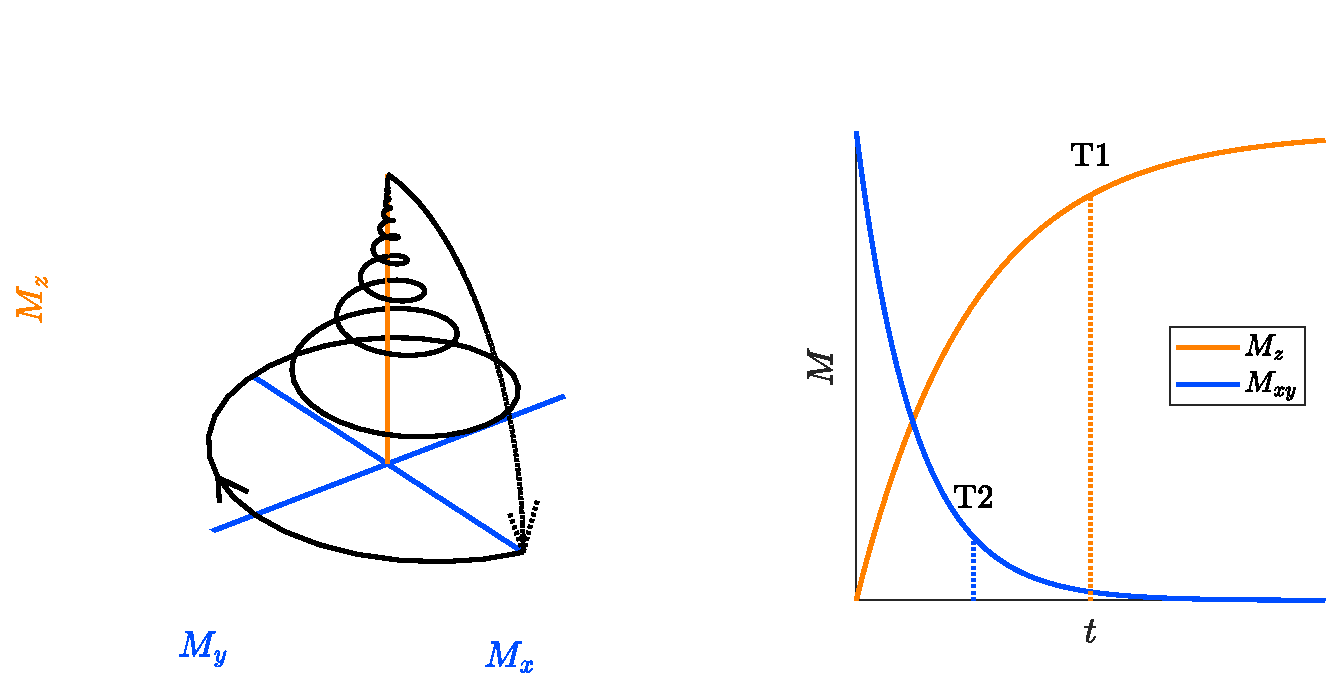
\includegraphics[width=\plotwidth]{mridecay3d}
  \caption{Visualization of T1 and T2 relaxation}
  \label{fig:mridecay3d}
\end{figure}
In an MR scanner, a powerful magnetic field induces alignment of proton dipoles with the field. Only a tiny fraction of the total protons align, but they create a small magnetic field $M_z$ which is distinct from the main field \cite{Bloch1946}. The aligned protons also rotate about the axis of alignment, imperfectly, like a spinning top; this is called precession, and the frequency of rotation is roughly homogeneous and proportional to the main field strength \cite{Bloch1946}. If a second magnetic field is applied which is $90^{\circ}$ perpendicular to the first, and rotating at the precession frequency, the aligned protons can be forced into temporary alignment with this transverse rotating field, before decaying back towards their original state, as illustrated in Figure \ref{fig:mridecay3d} \cite{Bloch1946}. This transient applied magnetic field is induced by a radio frequency (RF) pulse, and the rate at which the original magnetization $M_z$ is regained is described by the tissue-specific T1 relaxation constant,
\begin{equation}
M_z = M_0\et\left(1-e^{-\left(\frac{t}{T1}\right)}\right)\label{eq:T1}.
\end{equation}
The T1 constant is dictated by the ability of protons in the tissue to transfer energy to bonded atoms and surrounding molecules, since this energy transfer defines the transition from the high energy transverse state to the low energy original state \cite{Bloch1946,Bryant2005}. Large macromolecules, membranes, and lipids are generally able to facilitate this energy transfer more effectively than small molecules like water, producing a shorter T1 \cite{Koenig1990}. For this reason, myelinated WM has a shorter T1 than GM, which in turn has a shorter T1 than CSF, which is mostly water \cite{Roberts2007}.
\par
The rate of decay of the transverse moment $M_{xy}$ is actually not equal to the rate of regeneration of $M_z$. Rather, this is governed by the T2 relaxation constant,
\begin{equation}
M_{xy} = M_0\et\left(e^{-\left(\frac{t}{T2}\right)}\right)\label{eq:T2},
\end{equation}
which is always shorter that T1. This is because, in addition to T1 effects, the net rotating moment $M_{xy}$ is eroded by proton dephasing. When precessing protons, having a net dipole, interact with other dipoles or charged particles, their rotational frequency can be increased or decreased, but overall less coherent, reducing the perceptible net magnetization $M_{xy}$ \cite{Bloch1946}. In highly structured tissues like GM and WM, these interactions are more variable, dephasing is faster, and T2 is shorter \cite{Roberts2007}. In fluid environments like CSF, proton interactions are more homogeneous, yielding longer T2 \cite{Roberts2007}. For this reason, T2-weighted images are especially useful in identifying pathologies which degrade tissue structure, since they will have abnormally high T2 \cite{Roberts2007}. Both relaxation constants depend in a small way on the main magnetic field strength, measured in Tesla (T); T1 and T2 values for various brain tissues at 1.5T are summarized in Table \ref{tab:t1t2tissues}.
\par
\begin{table}
  \caption{T1 and T2 constants for brain tissues at 1.5 Tesla.}
  \label{tab:t1t2tissues}
  \centering{\setlength{\tabcolsep}{2pt}
  \begin{tabular}{ccrclcrclcrclcl}\hline
    Tissue && \multicolumn{3}{c}{T1 (ms)} && \multicolumn{3}{c}{T2 (ms)} && \multicolumn{3}{c}{$K [H]$ (a.u.)}&& Ref\\\hline
    WM  &&  719 & $\pm$ &  33 &&   73 & $\pm$ &   6 && 0.81 & $\pm$ & 0.03 && \cite{Schmitt2004}\\
    GM  && 1165 & $\pm$ &  88 &&   92 & $\pm$ &  11 && 0.98 & $\pm$ & 0.07 && \cite{Schmitt2004}\\
    CSF && 3337 & $\pm$ & 111 && 2562 & $\pm$ & 123 && 1.00 & $\pm$ & 0.07 && \cite{Schmitt2004}\\
    WML && 1124 & $\pm$ & 372 &&  136 & $\pm$ &  79 &&      &  $-$  &      && \cite{Stevenson2000}\ss{a}\\
    \hline
  \end{tabular}}\\[0.5em]
  \footnotesize{\ss{a} Estimated from Fig 1 supratentorial data (numerical results not given); $\pm$ IQR, not SD.}
\end{table}
Image acquisition involves sensing the transverse magnetization $M_{xy}$ following proton excitation by an RF pulse. The problem is that this small signal decays very quickly due to proton dephasing, which occurs even faster than $T2$ would predict due to a third factor, inhomogeneity in the main magnetic field \cite{Chavhan2009}. The time constant for this decays is termed $T2^*$, and its effects are usually undesirable \cite{Chavhan2009}. As a result, $M_{xy}$ is easily overpowered by the magnetic moment from the RF pulse, even after it is turned off, due to resonance. An important solution to this, called the spin-echo, was proposed by Erwin Hahn in \citeyear{Hahn1950} \cite{Hahn1950}. If $T2^*$ for each proton is assumed to be constant, then reversing the direction of rotation at a time $t$ should cause all protons to align again at exactly $2t$. Therefore, at $2t$ the transverse magnetization $M_{xy}$ -- the image signal -- manifests again for sensing, no longer confounded by RF coil resonance \cite{Hahn1950}.
\par
This second signal is called the Spin Echo ($SE$), and the interval $2t$ is termed the echo time ($TE$). Reversing the direction of rotation can be achieved by a $180^{\circ}$ RF pulse at time $TE/2$, in the same way the original excitation is achieved using a $90^{\circ}$ RF pulse (amount of rotation is proportional to the energy of the pulse). Acquisition of an entire image requires repetitions of this sequence with an interval called the repetition time ($TR$). An example spin echo sequence, showing $TE$ and $TR$, as well as $T1$ and $T2$ decay, is illustrated in Figure \ref{fig:mrispinecho}. Spatial encoding for creation of 2D and 3D images requires the use of additional electromagnetic gradients; however this topic is omitted here since it is quite involved, and not essential to the current work\footnote{The interested reader is directed to this comprehensive resource on the topic: \hreftt{http://mri-q.com/}}.
\par
\begin{figure}
  \centering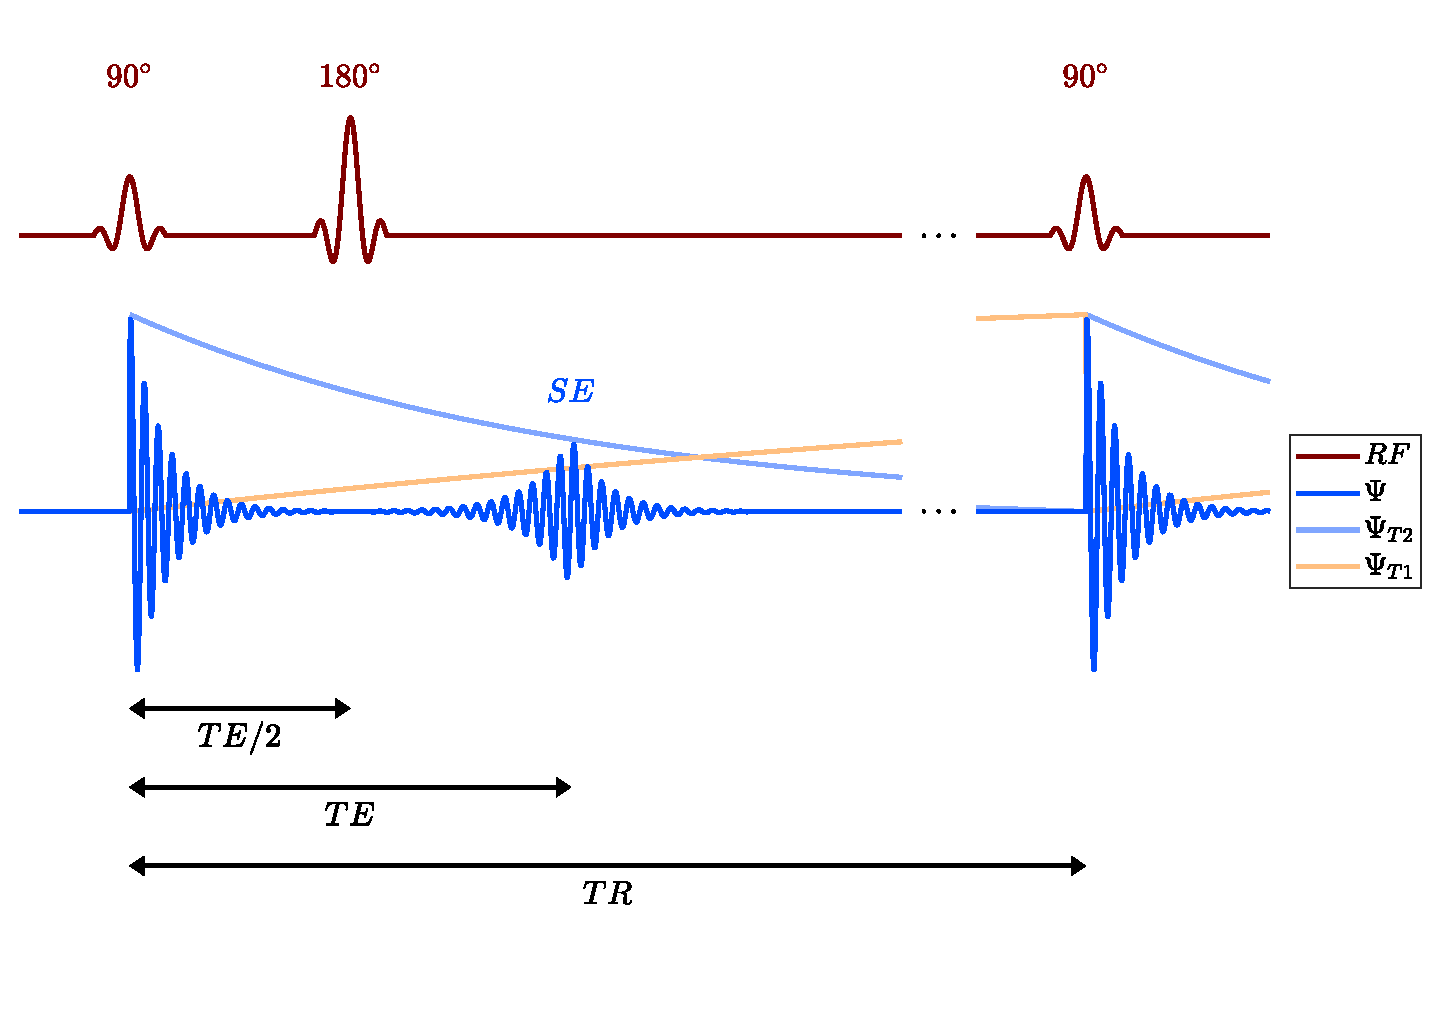
\includegraphics[width=\plotwidth]{mrispinecho}
  \caption{RF and MR signal for a basic Spin Echo sequence}
  \label{fig:mrispinecho}
\end{figure}
Using these principals, the nature of MR image contrast can finally be understood. In particular, the signal intensity $\Psi$ for a spin echo sequence at location $x$ can be described by the following 3-term equation,
\begin{equation}\label{eq:MRI-SE}
\Psi_{SE}(x) = \bigg[K [H](x)\bigg]\bigg[e^{-\left(\frac{TE}{T2(x)}\right)}\bigg]\bigg[1 - e^{-\left(\frac{TR}{T1(x)}\right)}\bigg],
\end{equation}
where $K$ is scaling factor, and $\left[H\right]$ denotes the proton density. If $TR$ is chosen to be relatively long, then the longitudinal magnetization $M_z$ is allowed to recover completely after each repetition, the third term tends towards 1 for all tissues, and differences in tissue specific $T1$ are nullified. Similarly, if $TE$ is relatively short, then $M_{xy}$ has little time to dephase, the second term is maintained close to 1, and differences in $T2$ are nullified. In order to emphasize differences in $T1$, therefore, $TR$ can be chosen shorter; for $T2$-weighted contrast, $TE$ can be chosen longer; and if differences in $[H]$ (proton density, PD) are to be emphasized, $TR$ can be kept long and $TE$ short. An example MRI slice using each of these image sequences is shown in Figure \ref{fig:4mri}, a--c.
\par
For identifying WML, T2-weighted images were conventionally used, since the pathology appears bright. However, CSF in the sulci and ventricles also appears bright on T2 images, making delineation of lesions -- especially periventricular lesions -- difficult in T2 images (Figure \ref{fig:4mri} b). To solve this problem, an adaptation of the usual RF pulse sequence can be used, called an inversion recovery (IR) \cite{Bydder1985}. In this sequence, an additional $180^{\circ}$ inverting RF pulse is added before the $90^{\circ}$ pulse, so that the longitudinal magnetization $M_z$ is inverted, then recovers to the original state, passing for a brief moment through zero net magnetization. The rate of recovery is governed by $T1$, so it is tissue specific. Furthermore, if the $90^{\circ}$ pulse is applied at the instant of zero net magnetization, no transverse moment will develop, nor the subsequent spin echo. Therefore this time interval, called the inversion time ($TI$), can be chosen to null the signal from any tissue with a unique $T1$. The equation governing the image signal simply adds an inversion term,
\begin{equation}\label{eq:MRI-IR}
\Psi_{IR}(x) = \bigg[K \left[H(x)\right]\bigg]\bigg[e^{-\left(\frac{TE}{T2(x)}\right)}\bigg]\bigg[1 + e^{-\left(\frac{TR}{T1(x)}\right)} - 2e^{-\left(\frac{TI}{T1(x)}\right)}\bigg].
\end{equation}
This inversion principal is now often used to null the signal from CSF, especially for delineation of WMH, in a sequence called FLuid Attenuation Inversion Recovery (FLAIR) \cite{Hajnal1992}. Figure \ref{fig:4mri} d shows an example FLAIR image, where a WMH can be seen, posterior to the occipital horn of the left lateral ventricle, much more clearly than in the T2 image.
\begin{figure}
  \centering
  \begin{subfigure}{0.24\textwidth}\includegraphics[width=\textwidth]{i15_training01_01_mprage.png}\caption{T1}  \end{subfigure}
  \begin{subfigure}{0.24\textwidth}\includegraphics[width=\textwidth]{i15_training01_01_t2.png}\caption{T2}      \end{subfigure}
  \begin{subfigure}{0.24\textwidth}\includegraphics[width=\textwidth]{i15_training01_01_pd.png}\caption{PD}      \end{subfigure}
  \begin{subfigure}{0.24\textwidth}\includegraphics[width=\textwidth]{i15_training01_01_flair.png}\caption{FLAIR}\end{subfigure}
  \caption{Example MRI image set with WMH pathology; from \cite{WMHSEG2017}}
  \label{fig:4mri}
\end{figure}
% ==================================================================================================
\subsection{MRI in White Matter Disease}
MR imaging of white matter lesions plays several important roles in management and research of white matter diseases. 
\par
In disease diagnosis, WMH are perhaps most important in 



Uniquely, MS lesions also manifest in the spinal cord, though this is beyond the scope of the MR images considered here.

Stroke, as an acute injury, does not fall under the usual diagnostic paradigm. 

Surprisingly, while WMH have been significantly associated with vascular 

they are not routinely included in dementia 

\cite{Debette2010}




+ research: as endpoint for clinical trials:
  - MS:
  - Alz:
  - Dem:
  - Stroke:
+ Disease diagnosis:
  - MS: \cite{Polman2011}
  - AD: The main guidelines for diagnosis are strictly clinical (i.e. exclude all imaging modalities and CSF assays) \cite{McKhann2011}.
  Yet, this omission may highlight the difficulty of large scale correlational studies of AD and WML.
  - Dem: (vascular only) 
  - Stroke:
+ Disease management:
  - MS:
  - Alz:
  - Dem:
  - Stroke:

a \citeyear{Debette2010} meta-analysis found that WMH in brain MRI were independently correlated with association of stroke risk


In all studies reviewed by \citeauthor{Debette2010}, however, WML were independently associated with stroke risk after controlling for vascular risk factors \cite{Debette2010}.



\clearpage
MR imaging of WMH plays several roles in management of MS and dementia, including diagnosis \cite{Polman2011,McKhann2011} and evaluation of new treatment efficacies \cite{Miller1996,Fahrbach2013,Sormani2013,Debette2010a}. In fact, it has been reported that MR imaging is up to ten times more sensitive to new lesion appearance than clinical symptoms in relapse remitting MS \cite{ORiordan1998}. In a \citeyear{Debette2010} meta-analysis, WM lesions were also associated with significantly increased risk of stroke and dementia, including AD \cite{Debette2010}, findings which have inspired several large-scale MRI-focused studies of these diseases, including the Canadian Atherosclerosis Imaging Network (CAIN) \cite{Tardif2013a} and the Alzheimer's Disease Neuroimaging Initiative (ADNI) \cite{Mueller2005}.
\par
Typically, analysis of WM lesions on MRI is performed manually, using specific criteria \cite{Polman2011,McKhann2011}, visual scales \cite{Pantoni2002}, or manual delineation \cite{Egger2017}. Manual delineation is most informative, providing both volumetric lesion load (LL) and exact spatial distribution of lesions. However, this approach is laborious, and is subject to large inter- and intra-rater variability. Such variability has been quantified in several works using similarity index (SI) and interclass correlation coefficient (ICC) (c.f. \ref{ss:metrics} for definitions); Table \ref{tab:interrater-cite} gives a summary of these results. Such discrepancies have motivated the development of automated segmentation tools in order to provide more consistent segmentations. These efforts have been further stimulated by the collection of large imaging databases (e.g. CAIN \& ADNI) for which manual delineation of lesions would be too time consuming.

%%%%%%%%%%%%%%%%%%%%%%%%%%%%%%%%%%%%%%%%%%%%%%%%%%%%%%%%%%%%%%%%%%%%%%%%%%%%%%%%%%%%%%%%%%%%%%%%%%%%
\section{Problem Statement}
White matter hyperintensities, as ubiquitous biomarkers of several diseases with unsolved pathophysiology, are of great interest to brain researchers. However, the current methods of quantifying WMH 

\cite{Polman2011,Pantoni2002,Egger2017}.


There are several manual rating scales which have been proposed \cite{Fazekas1987,VanSwieten1990,Scheltens1993,Ylikoski1993,Manolio1994}


Indeed, the majority of rating scales distinguish between deep (DL) and periventricular lesions (PVL) \cite{Kim2008}.

Problem Statement:
Advantages of segmentation over rating scales:
- Finer resolution
- Explicit spatial results, which can be correlated with 
Advantages of automated segmentation over manual segmentation:
- Perfect repeatability -- versus significant intra-/inter-rater variability
- Less time to perform the segmentation



\begin{table}[h]
  \caption{Reported mean inter-rater agreement measures for manual WMH segmentation}
  \centering
  \begin{tabular}{ccccc}
    \hline
    Ref                  & Raters & Data       & SI   & ICC \\
    \hline
    \cite{Steenwijk2013} &      2 & 120 slices & 0.83 & 0.96 \\
    \cite{DeBoer2009b}   &      2 & 6 images   & 0.75 & ---  \\
    \cite{Harmouche2006} &      5 & 10 images  & 0.64 & ---  \\
    \cite{Egger2017}     &      3 & 50 images  & 0.66 & 0.97 \\
    \hline
  \end{tabular}
  \label{tab:interrater-cite}
\end{table}

% ==================================================================================================
\subsection{Objective}
The primary objective of this thesis is to develop an algorithm for fully automatic segmentation of WMH, using FLAIR MRI alone. Secondary objectives include:
\begin{itemize}
  \item analysis of the limitations of prior work in this area;
  \item characterization of the important features for WMH segmentation;
  \item exploration and definition of appropriate cross validation techniques for the task;
  \item validation of the proposed algorithm on a large and heterogeneous database of FLAIR images.
\end{itemize}
% ==================================================================================================
\subsection{Challenges to Automatic Segmentation}\label{ss:autochallenges}
Human interpretation of MRI does has several advantages. 

Expert knowledge and understanding of image artifacts usually allows radiologists to distinguish WML from healthy tissues a with relative ease. 

\begin{enumerate}[itemsep=0pt,topsep=0pt]
  \item overlapping graylevel distributions of WMH and healthy tissues;
  \item bias field artifact, which can confound pathological hyperintensities \cite{Wardlaw2015};
  \item delineating the boundaries of focal lesions surrounded by DAWM \cite{Ge2003};
  \item identifying small WMH in MRI with significant partial volume effect due to large slice thickness \cite{Khademi2012};
  \item differentiating WMH from image artifacts \cite{Wardlaw2015};
  \item image variability.
\end{enumerate}
Confounding artifacts and pathologies include \cite{Wardlaw2015}:
\begin{itemize}[itemsep=0pt,topsep=0pt]
  \item CSF flow artifacts;
  %  \item Recent small subcortical infarcts;
  \item Perivascular spaces;
  \item Motion artifacts;
\end{itemize}
We will take ``image'' to mean one subject-scan, which may include several MRI sequences, and we take ``image variability'' to comprise:
\begin{itemize}[itemsep=0pt,topsep=0pt]
  \item differences in image contrasts (i.e. tissue intensity distributions), due to selection of MRI parameters;
  \item differences in image resolution (voxel size);
  \item differences in MRI scanner, including field strength and proprietary image reconstruction;
  \item inter-subject anatomical variability and lesion heterogeneity.
\end{itemize}

%%%%%%%%%%%%%%%%%%%%%%%%%%%%%%%%%%%%%%%%%%%%%%%%%%%%%%%%%%%%%%%%%%%%%%%%%%%%%%%%%%%%%%%%%%%%%%%%%%%%
\section{Prior Work}
Our endeavour is far from original. Efforts to automate segmentation of WMH date back to \citeyear{Kapouleas1990} \cite{Kapouleas1990} and the task has been the subject of several major reviews in \citeyear{Llado2012} \cite{Llado2012}, \citeyear{Garcia-Lorenzo2013} \cite{Garcia-Lorenzo2013}, and \citeyear{Caligiuri2015} \cite{Caligiuri2015}. The task has also been featured in four international competitions at the MICCAI (Medical Image Computing and Computer Assisted Intervention) Conference (2008 \cite{MSSEG2008}, 2016 \cite{MSSEG2016}, and 2017 \cite{WMHSEG2017}), and the ISBI (International Symposium on Biomedical Imaging) Conference (2015 \cite{MSISBI2015}), in which researchers vie to produce the best segmentation algorithms (c.f. \ref{ss:competitions}). A summary of the proposed approaches -- which is likely incomplete -- is given in Table \ref{tab:wmlsegtable}\footnote{A more detailed and interactive version of this table is available at \hreftt{www.uoguelph.ca/\~jknigh04/wmlseg/table.html}}. Below, the most important contributions in this area are introduced and summarized.
\begin{table}
  \caption{Summary of previous approaches to WMH segmentation with respect to image variability and reported performance (SI).}
  \footnotesize{\centering{\input{wmlsegtable}}}
  \label{tab:wmlsegtable}
\end{table}
% ==================================================================================================
\subsection{Segmentation Models}
Segmentation models represent a mapping from the content of an observed image to an image of labels or classes -- in this case, tissues. The output class image comprises an estimated label for each observed voxel, or, in probabilistic models, the probability of each class for each voxel. As in many classification problems, models can be described as either supervised or unsupervised. Supervised models have relatively large capacity to model arbitrary mappings, but learn a mapping relevant to the current task using feedback from labelled examples (i.e. by a human). Unsupervised models, by contrast, are usually problem-specific, and leverage prior knowledge and the image features to predict the label image; they do not require labelled data for optimization, at least in principle. 
\par
Features used for segmentation can be derived from individual voxels (e.g. graylevel), groups of voxels (e.g. local mean graylevel), the entire image (e.g. a histogram feature), spatial location (e.g. coordinates in a standardized space), or prior knowledge (e.g. class prior probability). It is useful to imagine the space spanned by all possible values of all features; this is called the feature space. Each observed voxel, having a unique value for each feature, therefore represents a unique location in this space. The task of segmentation is therefore to divide the feature space into subspaces corresponding to each class. In probabilistic models, these subspaces are better described as distributions of the class over the features.
% --------------------------------------------------------------------------------------------------
\subsubsection{Features}
Previous approaches to WMH segmentation have generally employed three types of features:
\begin{itemize}
  \item graylevel(s) of MRI sequence(s), often following a standardization step;
  \item prior tissue probability, often derived from a spatially coregistered prior image (e.g. ICBM \cite{Mazziotta2001});
  \item spatial location, often normalized to a common space;
\end{itemize}
Additional features are rarely used, since the combination of the above features are typically the only features employed by human raters.
% ==================================================================================================
\subsection{Proposed Methods}
The specific methods proposed for WMH segmentation are now reviewed.\footnote{This section copied verbatim from a paper in submission \cite{Knight2017a} -- is this allowed?}
% --------------------------------------------------------------------------------------------------
\subsubsection{Thresholding Techniques}
Since WMH are brighter than healthy brain tissue in FLAIR images, many unsupervised works have used thresholding of FLAIR intensities as the initial lesion segmentation.
For example, in the works by \citeauthor{Jack2001} \cite{Jack2001}, \citeauthor{DeBoer2009b} \cite{DeBoer2009b}, and \citeauthor{Smart2011}, \cite{Smart2011} optimal FLAIR thresholds are empirically estimated relative to histogram statistics, though \citeauthor{DeBoer2009b} use only estimated GM voxels in the histogram.
\citeauthor{Gibson2010} use a conservative FLAIR threshold initially, but then classify the remaining voxels using Fuzzy C Means clustering \cite{Gibson2010}.
\citeauthor{Samaille2012} use nonlinear diffusion filtering and watershed segmentation, before classifying candidate regions based on a FLAIR image threshold.
\citeauthor{Yoo2014} estimate the optimal threshold for FLAIR images using histogram statistics, derived from a regression model primarily considering the total lesion load \cite{Yoo2014}.
In works by \citeauthor{Khademi2014}, a peak in the conditional probability of edge content on graylevel is used to predict the transition between healthy tissue and lesion \cite{Khademi2014,Khademi2015,Knight2016a}.
\subsubsection{Mixture Models}
Most other unsupervised approaches are probabilistic models, often framed as a mixture model.
The work by \citeauthor{VanLeemput2001} \cite{VanLeemput2001} uses a similar framework as the early work by \citeauthor{Ashburner1997} \cite{Ashburner1997}, later incorporated into the SPM ``segment'' tool \cite{Ashburner2005}, which jointly estimates Gaussian graylevel distributions for each tissue class, and also bias field, using expectation maximization. In the model by \citeauthor{VanLeemput2001}, distribution parameters are estimated using outlier-insensitive estimators, and WMH are derived from model outliers using heuristic rules. The predicted classes are also smoothed spatially using a Markov Random Field (MRF).
\par
Similar works by \citeauthor{Bricq2008} \cite{Bricq2008}, \citeauthor{Schmidt2012} \cite{Schmidt2012}, \citeauthor{Jain2015} \cite{Jain2015}, and \citeauthor{Roura2015} \cite{Roura2015} use parametric mixture models to predict WMH as model outliers, and all but \cite{Roura2015} embed the model in a MRF.
\citeauthor{Khayati2008} \cite{Khayati2008} and \citeauthor{Subbanna2009} \cite{Subbanna2009} also use MRF-constrained mixture models, but model WMHs as a Gaussian-distributed tissue class, rather than as outliers.
In the works by \citeauthor{Harmouche2006}, parametric distributions are also used to model lesions, but such distributions are parameterized independently per brain region, in order to reflect lobe heterogeneity; a MRF is again used for regularization \cite{Harmouche2006,Harmouche2015}.
\citeauthor{Schwarz2009} again employ a Bayesian MRF model, but use lognormal distributions for WM and WMH \cite{Schwarz2009}.
\citeauthor{Souplet2008} use an augmented mixture model which includes partial volume averaging classes and an outlier class to perform initial brain tissue segmentation; WMH are subsequently classified using a FLAIR intensity threshold after contrast enhancement \cite{Souplet2008}. 
The work by \citeauthor{Herskovits2008} is much the same, but uses statistical information from training data to classify lesions (i.e. it is supervised) \cite{Herskovits2008}.
More recently, Graph-Cuts have been used in conjunction with mixture models, as in the works by \citeauthor{Garcia-Lorenzo2009} \cite{Garcia-Lorenzo2009}, \citeauthor{Tomas-Fernandez2015} \cite{Tomas-Fernandez2015}, and \citeauthor{Strumia2016} \cite{Strumia2016}.
\par
The Lesion-TOADS method by \citeauthor{Shiee2010} \cite{Shiee2010}, a lesion-specific adaptation of the TOADS algorithm \cite{Bazin2008}, presents an entirely new non-Gaussian paradigm for modelling class distributions, and incorporates topological energies in the objective function.
Other proposed unsupervised methods have used clustering by Fuzzy C-Means, including the works by \citeauthor{Admiraal-Behloul2005} \cite{Admiraal-Behloul2005}, \citeauthor{Gibson2010} \cite{Gibson2010}, and \citeauthor{Valverde2016} \cite{Valverde2016}.
\subsubsection{Classic Supervised Methods}
Many early supervised methods used K-Nearest Neighbours (K-NN) for voxel-wise WMH classification.
\citeauthor{Anbeek2005} used a K-NN model with features derived from spatial coordinates and voxel intensities from several modalities \cite{Anbeek2004,Anbeek2005}.
In the works by \citeauthor{Wu2006} \cite{Wu2006}, \citeauthor{Steenwijk2013} \cite{Steenwijk2013}, and \citeauthor{Fartaria2015} \cite{Fartaria2015}, spatial coordinates are substituted for tissue priors as K-NN features.
In the recently proposed BIANCA algorithm by \citeauthor{Griffanti2016} \cite{Griffanti2016}, spatial coordinates are added back, along with some patch-based features.
\par
Other works have also explored Support Vector Machines (SVM) for classification.
The works by \citeauthor{Lao2006} \cite{Lao2006}, \citeauthor{Abdullah2012} \cite{Abdullah2012}, and \citeauthor{Scully2010} \cite{Scully2010} each use a selection of intensity features, neighbouring intensities, tissue priors, morphological, and texture features with an SVM classifier.
Several more recent works have used decision tree-based classifiers, including Random Forest (RF) and AdaBoost.
\citeauthor{Akselrod-Ballin2009} \cite{Akselrod-Ballin2009} employ over 30 features for multi-scale image representation and classify voxels using RF.
Both \citeauthor{Geremia2011} \cite{Geremia2011} and \citeauthor{Roy2015} \cite{Roy2015} use a combination of intensity and tissue prior features to train a RF classifier, whereas \citeauthor{Wels2008} \cite{Wels2008} use a large number of Haar-like features to train an AdaBoost model.
\par
Logistic regression models have also gained popularity recently.
In the OASIS model by \citeauthor{Sweeney2013} \cite{Sweeney2013}, image intensities from T1, T2, PD, and FLAIR sequences are used individually, in multiplicative combination, and with Gaussian blurring as predictors for a global set of logistic regression parameters.
In the work by \citeauthor{Zhan2017} \cite{Zhan2017}, a similar logistic model is fitted using only the raw T1, T2, and FLAIR intensities, while bias correction is performed as preprocessing and spatial smoothness using MRF post processing.
In the work by \citeauthor{Dadar2017} \cite{Dadar2017}, spatial and intensity features from a flexible selection of MR sequences are used to train a linear regression model, the results of which are thresholded to give the lesion prediction.
Still more works have proposed other supervised models, including nonparametric Parzen classifiers \cite{Sajja2006}.
\subsubsection{Deep Learning}
A number of deep learning approaches have also been proposed, though their permeation in this problem space is surprisingly limited.
Both \citeauthor{Zijdenbos2002} \cite{Zijdenbos2002} and \citeauthor{Dyrby2008} \cite{Dyrby2008} train fully-connected voxel-wise Neural Networks with a selection of intensity, spatial, and tissue prior features to predict the lesion class.
In contrast, \citeauthor{Brosch2015} \cite{Brosch2015} construct a more modern deep convolutional model, which is capable of capturing both local and global dependencies.
\subsubsection{External Toolboxes}
Many of the proposed methods use registration, brain extraction, bias field correction, and segmentation tools available in freely available toolkits; these include the SPM\footnote{\hreftt{http://www.fil.ion.ucl.ac.uk/spm/}} toolkit
\cite{Sajja2006,Dyrby2008,Akselrod-Ballin2009,Smart2011,Schmidt2012,Yoo2014,Roy2015,Valverde2016} and the
FSL\footnote{\hreftt{https://fsl.fmrib.ox.ac.uk/fsl/}} toolkit
\cite{Herskovits2008,Gibson2010,Datta2013,Steenwijk2013,Sweeney2013,Roy2015,Wang2015,Griffanti2016,Zhan2017},
as well as bias correction by the
N3/4
%\footnote{\hreftt{https://www.slicer.org/wiki/Documentation/4.6/Modules/N4ITKBiasFieldCorrection}} 
\cite{Tustison2010}
algorithm
\cite{Zijdenbos2002,Harmouche2006,Fartaria2015,Guizard2015,Harmouche2015,Mechrez2016,Valverde2016,Dadar2017,Zhan2017}.
% --------------------------------------------------------------------------------------------------
%\subsubsection{Probabilistic Frameworks}
%Two of the most popular free segmentation tools for healthy brain MRI,
%``Segment'' in SPM\footnote{\hreftt{http://www.fil.ion.ucl.ac.uk/spm/}} \cite{Ashburner2005}
%and
%``FAST'' in FSL\footnote{\hreftt{https://fsl.fmrib.ox.ac.uk}} \cite{Zhang2001},
%employ a common mixture model framework which is estimated using expectation maximization (EM). These frameworks have been adapted in many works to segment WMH, either as model outliers, or as a new tissue class. Therefore, 
%The probability of class $k$ at location $i$, given the graylevel $y$ and model parameters $\bm{\theta}$, is 
%\begin{equation}
%  P(c_i=k \mid y_i, \bm{\theta}) = \frac{P(y_i, c_i=k \mid \bm{\theta})}{P(y_i \mid \bm{\theta})}
%\end{equation}
% ==================================================================================================
\subsection{Limitations}\label{ss:priorlimits}
Despite over 50 proposed algorithms and 

No 




Examples of hyperparameters in unsupervised models which can be over-tuned to the developmental dataset:
\begin{itemize}
  \item Outlier definition (Mahalanobis Distance)
  \item Histogram threshold definition.
\end{itemize}

However, 

(c.f. \ref{s:CVframeworks})


\clearpage
%%%%%%%%%%%%%%%%%%%%%%%%%%%%%%%%%%%%%%%%%%%%%%%%%%%%%%%%%%%%%%%%%%%%%%%%%%%%%%%%%%%%%%%%%%%%%%%%%%%%
\section{Contributions}
The major contributions of this thesis are as follows:
\begin{enumerate}
  \item A review and critique of the previously proposed WMH segmentation algorithms;
  \item Leave-One-Source-Out Cross Validation (LOSO-CV): a validation framework which accurately characterizes the generalization performance of medical image analysis methods;
  \item A new FLAIR-only WMH segmentation algorithm;
  \item Extensive validation of the proposed method and its components.
\end{enumerate}
The remainder of this thesis is organized as follows:
Chapter 2 motivates and develops the voxel-wise logistic regression model, including expected challenges and solutions with this approach;
Chapter 3 explores optimization of model components through experiment, and then presents segmentation performance results under various cross validation schemes;
Chapter 4 discusses the performance results, summarizes the contributions, and highlights avenues of future work.
% --------------------------------------------------------------------------------------------------
% ==================================================================================================
%%%%%%%%%%%%%%%%%%%%%%%%%%%%%%%%%%%%%%%%%%%%%%%%%%%%%%%%%%%%%%%%%%%%%%%%%%%%%%%%%%%%%%%%%%%%%%%%%%%%

  %%%%%%%%%%%%%%%%%%%%%%%%%%%%%%%%%%%%%%%%%%%%%%%%%%%%%%%%%%%%%%%%%%%%%%%%%%%%%%%%%%%%%%%%%%%%%%%%%%%%
% ==================================================================================================
% --------------------------------------------------------------------------------------------------
\chapter{Methodology}
In this section we introduce the proposed model and explore its parametrization.
\par
Wherever possible, concepts related to segmentation and classification will be described in their most general sense, since many of the conclusions presented here may also apply to other image analysis and machine learning tasks.
%%%%%%%%%%%%%%%%%%%%%%%%%%%%%%%%%%%%%%%%%%%%%%%%%%%%%%%%%%%%%%%%%%%%%%%%%%%%%%%%%%%%%%%%%%%%%%%%%%%%
\section{Motivation}

%Many of the previously proposed WMH segmentation algorithms predict the class of a voxel without any spatial information. In the absence of spatial information, 
%
%The work by \citeauthor{Khademi2012} \cite{Khademi2012,Khademi2014,Khademi2015} was particularly promising, since it overcame many of the usual requirements. These include: the use of multiple MRI modalities, which are not always available; image registration to a common space, which is never perfect and introduces interpolation artifact; the use of training data, which is difficult to find; and assumed Gaussian distribution of tissue graylevels, which is rarely valid.
%
%
%
%Assumptions which many models make, and whether they are wrong:
%
%- parametric modelling of graylevel distributions: with single Gaussians: almost certainly wrong. Confounding factors: PVA, parallel MRI signals, motion artifacts, 
%
%The most recent implementation of the EM-fit mixture model by \citeauthor{Ashburner2005} in \cite{Ashburner2005} permits a user-specified number of Gaussian distributions for each tissue class, 
%
%(though convergence is likely challenging)
%
%as well as 
%
%However, the central assumption of these methods is that the distributions of WMH graylevels do not overlap significantly with distributions of any other tissue class.
%
%However, it has been suggested that there is regional heterogeneity in relaxation rates of brain tissues \cite{Sled2004}, and that WMH intensity depends in part on location \cite{Stevenson2000}.

%%%%%%%%%%%%%%%%%%%%%%%%%%%%%%%%%%%%%%%%%%%%%%%%%%%%%%%%%%%%%%%%%%%%%%%%%%%%%%%%%%%%%%%%%%%%%%%%%%%%
\section{Proposed Model}
We now present the proposed model...
\par
The probability of the lesion class $c=1$ in one location $x$, given the features $\by = [y^1,\dots,y^\K]^T$  is modelled as a logistic function parameterized by a vector $\bb = [\b^1,\dots,\b^\K]^T$,
\begin{equation}
  P(c=1\mid\by,\bb) = \frac{1}{1+e^{-\bb^T\by}}
  \label{eq:model}
\end{equation}
This probability -- the estimated lesion label -- is denoted $\hat{c} = P(c=1\mid\by,\bb) \in [0,1]$.
\par
The assumptions of this model include the following:
\begin{itemize}[itemsep=0pt]
  \item only 2 tissues classes are modelled: WMH and healthy brain tissue;
  \item image graylevel(s) and spatial location are sufficient features to discriminate the two classes;
  \item in each voxel, the WMH class is monotonically separable from the healthy class by graylevel(s)
\end{itemize}
% ==================================================================================================
\subsection{Model Fitting}
Fitting the model involves estimating $\bb$ for each voxel $x$. This requires some training data: feature vectors from a population of $N$ observations $\bY = \{\by_1,\dots,\by_\N\}$, and the corresponding labels $\C = \{c_1,\dots,c_\N\}$. The optimal $\bb$ should maximize the likelihood of the model, given this data -- i.e. maximum likelihood estimation (MLE). If the training data are assumed to be independently observed, then the likelihood (conditioned on the data) is defined from binomial theory as 
\begin{align}
  L(\bb\mid\C,\bY) &= \prod_{n=1}^{N} P(c=1\mid\by_n,\bb)^{c_n} \left(1-P(c=1\mid\by_n,\bb)^{1-c_n}\right)\nonumber\\
  &= \prod_{n=1}^{N} \Big[\hat{c}_n^{\en c_n} \left(1-\hat{c}_n^{\en 1-c_n}\right)\Big]
  \label{eq:likelihood}
\end{align}
For computational reasons, it is simpler and asymptotically equivalent to maximize the log-likelihood,
\begin{align}
\L(\bb) &= \log{ \prod_{n=1}^{N} \Big[\hat{c}_n^{\en c_n} \left(1-\hat{c}_n^{\en 1-c_n}\right)\Big] }\nonumber\\
&= \sum_{n=1}^{N} \Big[ c_n \log \hat{c}_n + (1-c_n) \log (1-\hat{c}_n) \Big] \nonumber\\
&= \sum_{n=1}^{N} \Big[ c_n \bb^T\by_n - \log (1+e^{\bb^T\by_n}) \Big] 
\label{eq:loglikelihood}
\end{align}
The optimal $\bb$ is therefore resolved by maximizing the log-likelihood,
\begin{align}
\bb^* &= \underset{\bb}{\arg\max} \en\L(\bb)\nonumber\\
&= \underset{\bb}{\arg\max}\en\sum_{n=1}^{N} \Big[ c_n \bb^T\by_n - \log (1+e^{\et\bb^T\by_n}) \Big]
\label{eq:argmaxmle}
\end{align}
% --------------------------------------------------------------------------------------------------
\subsection{Iterative Updates}
Estimation of $\bb^*$ can be performed using iterative optimization, using an initial estimate $\bb^{(0)}$ and an update term $\Delta\bb^{(t)}$,
\begin{equation}
\bb^{(t+1)} \leftarrow \bb^{(t)} + \alpha\thinspace\Delta\bb^{(t)},
\label{eq:update}
\end{equation}
where $\alpha$ is a small valued learning rate parameter. There are many possible definitions of $\Delta\bb$, including simply the gradient of $\L(\bb)$, denoted $\nabla_{\bb}\L$. However, it can be shown that $\L(\bb)$ is convex, so higher order update equations can be used. The work by \citeauthor{Minka2003} \cite{Minka2003} compares several options, including Newton's method (and variants), conjugate gradient, iterative scaling (and variants), and dual optimization\footnote{Matlab code available at \hreftt{https://github.com/tminka/logreg/}}. For small feature dimensionality ($K$), performance differences among the options were small. Classic Newton updates gave a good balance between memory requirements and computational order, so they are used.
\par
If the gradient $\nabla_{\bb}\L$ and Hessian matrix $\nabla^2_{\bb}\L$ are defined as
\begin{align}
\nabla_{\bb}\L &= \left[\begin{array}{c}
\frac{\d L}{\d\b^1}\\\vdots\\\frac{\d L}{\d\b^\K}
\end{array}\right],\label{eq:llgradient0}\\
\nabla^2_{\bb}\L &= \left[\begin{array}{ccc}
\frac{\d^2 L}{\d\b^1\d\b^1}&\cdots&\frac{\d^2 L}{\d\b^1\d\b^\K}\\
\vdots&\ddots&\vdots\\
\frac{\d^2 L}{\d\b^\K\d\b^1}&\cdots&\frac{\d^2 L}{\d\b^\K\d\b^\K}
\end{array}\right]\label{eq:llhessian0},
\end{align}
then the Newton update is given by
\begin{equation}
\Delta\bb = -{\nabla^2_{\bb}\L}^{-1}\nabla_{\bb}\L.
\label{eq:newtonmle}
\end{equation}
In the current model, the gradient is given by 
\begin{equation}
\nabla_{\bb}\L = \sum_{n=1}^{N} \by_n\left(c_n - \hat{c}_n\right),
\label{eq:llgradient}
\end{equation}
and the Hessian by
\begin{equation}
\nabla^2_{\bb}\L = \sum_{n=1}^{N} \by_n{\by_n}^T \left(c_n - \hat{c}_n\right).
\label{eq:llhessian}
\end{equation}
Substituting (\ref{eq:llgradient}) and (\ref{eq:llhessian}) into (\ref{eq:newtonmle}), the explicit update  $\Delta\bb$ for (\ref{eq:update}) is obtained.
% --------------------------------------------------------------------------------------------------
\subsection{Implementation}

%%%%%%%%%%%%%%%%%%%%%%%%%%%%%%%%%%%%%%%%%%%%%%%%%%%%%%%%%%%%%%%%%%%%%%%%%%%%%%%%%%%%%%%%%%%%%%%%%%%%
\section{Bias Correction \& Registration}



%%%%%%%%%%%%%%%%%%%%%%%%%%%%%%%%%%%%%%%%%%%%%%%%%%%%%%%%%%%%%%%%%%%%%%%%%%%%%%%%%%%%%%%%%%%%%%%%%%%%
\section{Graylevel Standardization}

\clearpage
%%%%%%%%%%%%%%%%%%%%%%%%%%%%%%%%%%%%%%%%%%%%%%%%%%%%%%%%%%%%%%%%%%%%%%%%%%%%%%%%%%%%%%%%%%%%%%%%%%%%
\section{Regularization}
Even if perfect registration and graylevel standardization are achieved, three challenges remain for the VLR model. These challenges involve contradictions between prior knowledge and the MLE-fitted model using the available training data. That is, these challenges could all be overcome by a more complete training set, but this is usually not available. The three challenges are:
\begin{enumerate}
  \item \label{chmle:separable} \textbf{Separable classes:} 
  When data from two classes are perfectly separable, the MLE error surface in parameter space has a convex global minimum at infinity. As a result, the fitted logistic model in voxels with separable data approaches a step-function, since $\b^1\rightarrow+\infty$. This implies that on either side of a specific graylevel threshold ($\tau$), the model is either 100\% confident in predicting the non-lesion class, or 100\% confident in predicting the lesion class. In fact, no threshold is ever so perfect, and instead a level of uncertainty should be maintained around the decision boundary. These two cases are illustrated in Figure \ref{fig:chmle-sep}.
  \item \label{chmle:sparse} \textbf{Sparsely observed lesion class:} 
  Since WML are often distributed in consistent locations, many brain regions contain no lesions across the entire training dataset. In some locations (e.g. the GM), this is expected, while in others (e.g. juxtacortical WM) our prior knowledge predicts lesions will eventually be observed. As illustrated in Figure \ref{fig:chmle-noles}, the MLE-fitted model does not maintain the ability to predict $\hat{c} = 1$ in this location, regardless of the features. However, we would like to keep this ability in many of these locations. 
  \item \label{chmle:noisy} \textbf{Noisy parameter images:} 
  Modelling every voxel independently is risky. We assume that similar locations will contain similar training data, yielding smooth parameter images, which we expect. If this assumption is sometimes invalid, parameter images could contain noise or discontinuities, creating artifacts in estimated lesion class images.
\end{enumerate}
\begin{figure}
  \centering
  \begin{subfigure}{\plotwidth}
    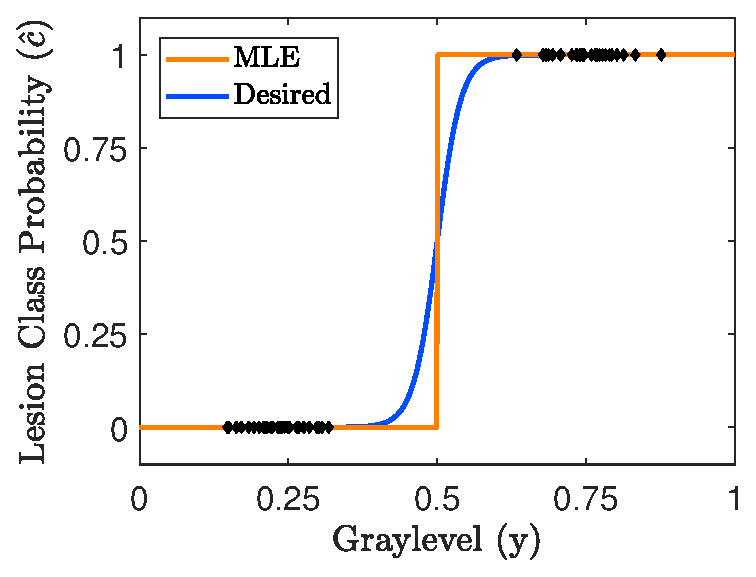
\includegraphics[width=\textwidth]{chmle-sep}\caption{Separable classes}\label{fig:chmle-sep}
  \end{subfigure}
  \begin{subfigure}{\plotwidth}
    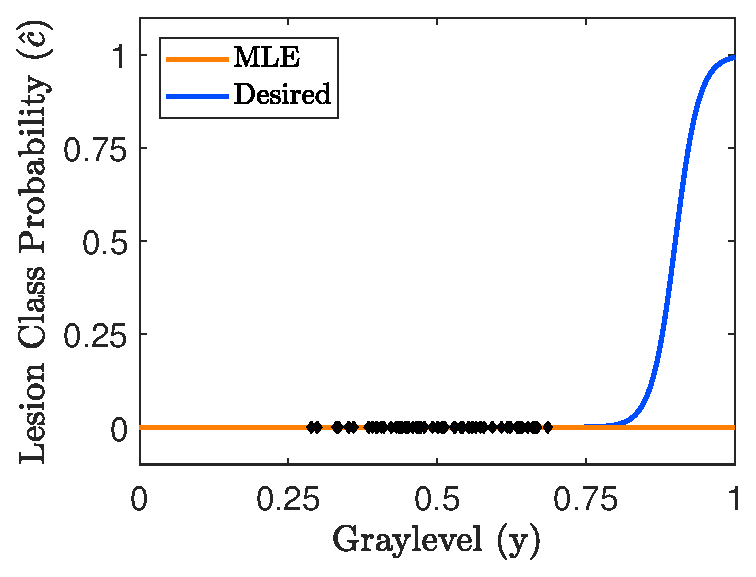
\includegraphics[width=\textwidth]{chmle-noles}\caption{No lesions}\label{fig:chmle-noles}
  \end{subfigure}
  \caption{Challenges encountered using ML estimation of a logistic model.}
  \label{fig:chmle}
\end{figure}
Solutions to these problems are called regularizations -- methods of injecting prior knowledge about the expected model into the optimization. Model fitting which includes regularizations is termed maximum a posteriori (MAP) estimation. Several regularization strategies are explored below.
% ==================================================================================================
\subsection{Data Augmentation}
Noting the central role of training data in each of the above challenges, methods of artificially increasing the training dataset size may be particularly useful in solving them. Data augmentation has long been used in machine learning tasks with limited training data, and there are several methods of generating synthetic data. In low dimensional input/output spaces, random sampling of fitted class-conditional posterior distributions can produce reasonable samples with known labels \cite{Tanner1987}. In higher dimensional problem spaces, however, imputation is more difficult \cite{Goodfellow2014}. For example, the space of potential $100\times100\times100$-sized images has $100^3$ dimensions (one per voxel), yet only a small inner subspace represents plausible images. Generating synthetic examples in this space is therefore challenging, especially for segmentation tasks, where the outputs have dimensionality roughly equal to the input.
\par
Alternatively, simple image manipulations can still afford model improvements \cite{Krizhevsky2012}. In segmentation tasks, both the input image(s) and the corresponding label images can be translated, reflected, rotated, and perhaps resized, thereby avoiding the generation of genuinely synthetic examples. In the current task, 

% ==================================================================================================
\subsection{Classic Regularization}
Challenge \ref{chmle:separable} is well-known in regression problems, and a good solution is to penalize the magnitude of model parameters using the $L_p$-norm: $\lambda\norm{\bb}_p$ \cite{Zou2005}. It can be shown that $L_1$ regularization corresponds to a Laplacian prior on elements of $\bb$, with scale parameter inversely proportional to $\lambda$ (equivalently, this assumes that the model error follows this distribution); similarly, $L_2$ regularization implies a Gaussian prior, with standard deviation inversely proportional to $\lambda$ \cite{Zou2005}. The penalty is appended to the objective function (\ref{eq:argmaxmle}), as in 
\begin{align}
\bb^* &= \J(\bb)\nonumber\\
&= \underset{\bb}{\arg\max}\en\L(\bb) - \lambda\norm{\bb}_p \nonumber\\
&= \underset{\bb}{\arg\max}\en\sum_{n=1}^{N} \Big[ c_n \bb^T\by_n - \log (1+e^{\et\bb^T\by_n}) \Big] - \lambda\norm{\bb}_p
\label{eq:argmaxmap}
\end{align}
Due to its relatively large gradient near zero, $L_1$ regularization is typically used to encourage sparsity in the feature weights (i.e. $\b^k\rightarrow0$) \cite{Tibshirani1996}. This is not necessarily desirable in our model. Moreover, the expansion of the $\norm{\bb}_1$ term in the gradient of the objective function is not straightforward, since it is non-differentiable at zero \cite{Tibshirani1996,Lee2006}. Conversely, $L_2$ regularization is more effective at limiting parameter magnitude -- which is the current aim -- and the first and second order gradients of (\ref{eq:argmaxmap}) derive easily \cite{Minka2003}. For these reasons, we consider only $L_2$ regularization, yielding the following change to the Newton update expression (\ref{eq:newtonmle}),
\begin{equation}
\Delta\bb = -{\left(\nabla^2_{\bb}\L-\lambda I\right)}^{-1}\left(\nabla_{\bb}\L-\lambda\bb\right)
\label{eq:newtonmap}
\end{equation}
What remains is to select an appropriate value of $\lambda$. This is explored experimentally using a toy model (cf. \ref{ss:toyreg}).
% ==================================================================================================
\subsection{Pseudo-Lesion}
%Challenge \ref{chmle:sparse} is less common, since discriminative models are rarely fit in the absence of one class altogether. 
%
%It is tempting to simply transfer samples from other spatial locations 
%
%sampling of the global posterior distribution of lesion graylevels
%
%
%
%However, it has been suggested that there is regional heterogeneity in relaxation rates of brain tissues \cite{Sled2004}, and that WMH intensity depends in part on location \cite{Stevenson2000}.


% ==================================================================================================
\subsection{Parameter Image Smoothing}
% Finally, 

%%%%%%%%%%%%%%%%%%%%%%%%%%%%%%%%%%%%%%%%%%%%%%%%%%%%%%%%%%%%%%%%%%%%%%%%%%%%%%%%%%%%%%%%%%%%%%%%%%%%
\section{Post-Processing}
% ==================================================================================================
\subsection{Markov Random Field}
%%%%%%%%%%%%%%%%%%%%%%%%%%%%%%%%%%%%%%%%%%%%%%%%%%%%%%%%%%%%%%%%%%%%%%%%%%%%%%%%%%%%%%%%%%%%%%%%%%%%
\section{Performance Metrics}
\label{ss:metrics}
Segmentation performance of the model is characterized in two respects: voxel-wise agreement and total lesion load (LL) volume agreement. Voxel-wise agreement is quantified using the following measures:
\begin{itemize}
  \item \textbf{Similarity Index (SI)} (\textsc{aka} Dice Similarity Coefficient, F1-Score)\\Measures overall segmentation performance.
  \begin{equation}SI = \dfrac{2TP}{2TP + FP + FN}\end{equation}
  \item \textbf{Precision (Pr)} (\textsc{aka} Overlap Fraction, Positive Predictive Value)\\Fraction of predicted predicted positives which are true positives.
  \begin{equation}Pr = \dfrac{TP}{TP+FP}\end{equation}
  \item \textbf{Recall (Re)} (\textsc{aka} Sensitivity, True Positive Rate)\\Fraction of true positives which are predicted positive.
  \begin{equation}Re = \dfrac{TP}{TP+FN}\end{equation}
\end{itemize}
Note that typical performance metrics like accuracy and sensitivity are avoided, since they include the $TN$ count in the numerator, which is typically much larger than $TP + FP + FN$ combined (i.e. lesions are a rare event). Volume agreement between segmentations is characterized using the 2-way mixed-effects single-rater absolute intraclass correlation coefficient (ICC)\footnotemark\ \cite{Koo2016}. Trends in in over/undersegmentation with lesion load are illustrated using Blant-Altman plots.
\footnotetext{Option \texttt{`A-1'} in the MATLAB function \texttt{ICC} from \hreftt{https://www.mathworks.com/matlabcentral/fileexchange/22099}}

%%%%%%%%%%%%%%%%%%%%%%%%%%%%%%%%%%%%%%%%%%%%%%%%%%%%%%%%%%%%%%%%%%%%%%%%%%%%%%%%%%%%%%%%%%%%%%%%%%%%
\section{Model Summary}



A summary of the model is shown in Figure \ref{fig:modelsum}.
\begin{figure}
  \centering\scalebox{0.65}{\pgfdeclarelayer{background}
\pgfdeclarelayer{foreground}
\pgfsetlayers{background,main,foreground}
\tikzset{%
  arrow/.style = { ->, >=Latex,  very thick, rounded corners, draw = #1!60!white },
  input/.style = { ->, >=Latex, ultra thick, rounded corners, draw = red },
  clr/.style   = { ultra thick, rounded corners, fill = #1!60!white },
  image/.style = { fill = black, draw = black!80!white, ultra thick, inner sep = 0 },
  plot/.style  = { fill = white, inner sep = 0 },
  label/.style = { fill = white, fill opacity = 0, text opacity = 1 },
  tbox/.style  = { fill = white, draw = #1!60!white, very thick, align = center }
  %  title/.style = { draw = #1!60!white, very thick, align = center, minimum width = 3.4 cm, minimum height = 1.2 cm, rotate=+90 },
  %  fun/.style   = { fill = black!10!white, draw=black, circle, minimum size = 2*\fw cm, inner sep = 0 },
}
\newcommand*{\img}[3]{%
  \node[image] at (#1,#2){\includegraphics[width=\ixx cm, height=\iyy cm]{#3}};
}
\newcommand*{\imgt}[4]{%
	\img{#1}{#2}{#3}
	\begin{pgfonlayer}{foreground}
		\node[label] at (#1,#2-\iy-0.4){\large #4};
	\end{pgfonlayer}
}
\newcommand*{\plot}[5]{%
  \node[plot] at (#1,#2){\includegraphics[width=#3cm, height= #4cm]{#5}};
}
\newcommand*{\voxpath}[4]{%
  \filldraw[fill=black!20!white,draw=black]
  (#1,#2)--(#1+\vw,#2)--(#1+#3,#2-#3+\vw)--(#1+#3-\vw,#2-#3+\vw)--(#1,#2);
  \filldraw[fill=black!20!white,draw=black]
  (#1,#2)--(#1,#2-\vw)--(#1+#3-\vw,#2-#3)--(#1+#3-\vw,#2-#3+\vw)--(#1,#2);
  \filldraw[fill=black!20!white,draw=black]
  (#1+#3,#2-#3)--(#1+#3,#2-#3+\vw)--(#1+#3-\vw,#2-#3+\vw)--(#1+#3-\vw,#2-#3)--(#1+#3,#2-#3);
  \node[below right] at (#1+#3,#2-#3) {#4};
}
\newcommand*{\imgstack}[5]{%
  \foreach \x in {0,...,#3}{\img{#1-0.1*#3+0.1*\x}{#2+0.1*#3-0.1*\x}{#4}}
  \begin{pgfonlayer}{foreground}
	  \node[label] at (#1,#2-\iy-0.4){\large #5};
	\end{pgfonlayer}{foreground}
}
\newcommand*{\imgvoxstack}[5]{%
	\voxpath{#1+\vw+0.3-0.1*#3-\vl-\vl}
					{#2-\vw-0.2+0.1*#3+\vl+\vl}{\vl}{}
	\imgstack{#1}{#2}{#3}{#4}{#5}
	\voxpath{#1+\vw+0.3}
	        {#2-\vw-0.2}{\vl}{}
}
\newcommand*{\textbox}[6]{%
  \node[tbox=#5,minimum width=#3cm,minimum height=#4cm]at(#1,#2){#6};
}
%\newcommand*{\blocktitle}[4]{%
%  \node[title=#3]at(#1,#2){#4};
%  \fill[clr=#3](#1+0.6,#2+1.7)--(#1+0.6,#2-1.7)--(#1+0.6+0.3,#2);
%}
\newcommand*{\vw}{0.1}
\newcommand*{\vl}{0.7}
\newcommand*{\ix}{0.8}\newcommand*{\ixx}{1.6}
\newcommand*{\iy}{1}  \newcommand*{\iyy}{2}
\newcommand*{\pw}{1.5}
\newcommand*{\fw}{0.3}

% --------------------------------------------------------------------------------------------------
\begin{tikzpicture}
    \useasboundingbox(1.5, 0.0) rectangle (24.0, 20.5);
    \begin{pgfonlayer}{background}
      % background boxes
      \draw[black!30!white,rounded corners,very thick](-0.25, 0.25) rectangle (23.75, 9.75);
      \draw[black!30!white,rounded corners,very thick](-0.25,10.25) rectangle (23.75,20.00);
      % box labells
      \node[fill=black!10!white,rounded corners,minimum width=3cm, minimum height=1.0cm]at(21.75,19.00){\textsc{Training}};
      \node[fill=black!10!white,rounded corners,minimum width=3cm, minimum height=1.0cm]at(21.75, 8.75){\textsc{Testing}};
      %\draw[step=0.5,black!10!white,very thin](-0.5, 0.0) grid (24.0,20.0);
    \end{pgfonlayer}
    % training
    \imgt       { 1.0}{18.0}{c1}{$C_1(x)$}
    \imgt       { 1.0}{14.0}{c2}{$C_{\textsc{n}}(x)$}
    \imgt       { 3.0}{18.0}{i1}{$Y_1(x)$}
    \imgt       { 3.0}{14.0}{i2}{$Y_{\textsc{n}}(x)$}
    \node[font=\fontsize{30}{0}\selectfont,align=center] at ( 1.0,15.8) {$\vdots$};
    \node[font=\fontsize{30}{0}\selectfont,align=center] at ( 3.0,15.8) {$\vdots$};
    \imgstack   {10.0}{16.0}{6}{ir} {$\mathcal{Y}(x)$}
    \imgvoxstack{13.0}{16.0}{6}{jr} {$\tilde{\mathcal{Y}}(x)$}
    \imgvoxstack{13.0}{12.0}{6}{c1} {$\mathcal{C}(x)$}
    \plot       {17.5}{14.0}{4}{4}  {lr-fit}
    \imgvoxstack{22.0}{14.0}{1}{bb} {$\bm{\beta}(x)$}
    % testing
    \imgstack   { 3.0}{ 2.0}{1}{bb} {$\bm{\beta}(x)$}
    \imgvoxstack{ 3.0}{ 6.0}{0}{it} {$Y_{test}(x)$}
    \imgvoxstack{10.0}{ 2.0}{1}{bb} {$\bm{B}(x)$}
    \imgvoxstack{10.0}{ 6.0}{0}{jt} {$\tilde{Y}_{test}(x)$}
    \plot       {14.5}{ 4.0}{4}{4}  {lr-test}
    \imgvoxstack{19.0}{ 4.0}{0}{qt} {$\hat{C}_{test}^*(x)$}
    \imgt       {22.0}{ 4.0}{lt}    {$\hat{C}_{test}(x)$}
    % training arrows
    \draw[arrow={blue}  ]( 3.0+\ix,18.0    )--( 3.5+\ix,18.0)--( 3.5+\ix,16.0)--( 5.0,16.0);
    \draw[arrow={blue}  ]( 3.0+\ix,16.0    )--( 5.0    ,16.0);
    \draw[arrow={blue}  ]( 3.0+\ix,14.0    )--( 3.5+\ix,14.0)--( 3.5+\ix,16.0)--( 5.0,16.0);
    \draw[arrow={blue}  ]( 8.0    ,16.0    )--(10.0-\ix,16.0);
    \draw[arrow={blue}  ]( 1.0    ,12.3    )--( 1.0    ,12.0)--( 5.0,    12.0);
    \draw[arrow={blue}  ]( 5.0    ,12.0    )--(13.0-\ix,12.0);
    \draw[arrow={blue},dotted](6.5,16.0    )--( 6.5    ,12.5);
    \draw[arrow={violet}](10.0    ,16.0+\iy)--(10.0    ,18.5);
    \draw[arrow={violet}](11.5,    19.0    )--(13.0    ,19.0)--(13.0,16.0+\iy);
    \draw[arrow={red}   ](13.0+\ix,16.0    )--(14.5    ,16.0)--(14.5,14.0)--(15.5,14.0);
    \draw[arrow={red}   ](13.0+\ix,12.0    )--(14.5    ,12.0)--(14.5,14.0)--(15.5,14.0);
    \draw[arrow={red}   ](19.5    ,14.0    )--(22.0-\ix,14.0);
    % testing arrows
    \draw[arrow={blue}  ]( 3.0+\ix, 6.0    )--( 5.0    , 6.0);
    \draw[arrow={blue},dotted](6.5, 6.0    )--( 6.5    , 2.5);
    \draw[arrow={blue}  ]( 3.0+\ix, 2.0    )--( 5.0    , 2.0);
    \draw[arrow={blue}  ]( 8.0    , 2.0    )--(10.0-\ix, 2.0);
    \draw[arrow={violet}]( 6.5    , 6.5    )--( 6.5    , 8.0);
    \draw[arrow={violet}]( 8.0    , 8.5    )--(10.0    , 8.5)--(10.0    , 6.0+\iy);
    \draw[arrow={red}   ](10.0+\ix, 6.0    )--(11.5    , 6.0)--(11.5, 4.0)--(12.5, 4.0);
    \draw[arrow={red}   ](10.0+\ix, 2.0    )--(11.5    , 2.0)--(11.5, 4.0)--(12.5, 4.0);
    \draw[arrow={red}   ](16.5    , 4.0    )--(19.0-\ix, 4.0);
    \draw[arrow={orange}](19.0    , 4.0+\iy)--(19.0    , 6.5);
    \draw[arrow={orange}](20.5,     7.0    )--(22.0    , 7.0)--(22.0, 4.0+\iy);
    % training texts
    \textbox    { 6.5}{16.0}{3}{1.0}{blue}  {Bias Correction\\\& Registration}
    \textbox    { 6.5}{12.0}{3}{1.0}{blue}  {Same Transform\\Applied}
    \textbox    {10.0}{19.0}{3}{1.0}{violet}{Histogram\\Matching}
    \textbox    {17.5}{17.0}{4}{1.0}{red}   {Logistic Regression\\Model Fitting}
    % testing texts
    \textbox    { 6.5}{6.25}{3}{0.5}{blue}  {Bias Correction}
    \textbox    { 6.5}{5.75}{3}{0.5}{blue}  {Registration}
    \textbox    { 6.5}{ 2.0}{3}{1.0}{blue}  {Inverse Transform\\Applied}
    \textbox    { 6.5}{ 8.5}{3}{1.0}{violet}{Histogram\\Matching}
    \textbox    {14.5}{ 7.0}{4}{1.0}{red}   {Logistic Regression\\Lesion Prediction}
    \textbox    {19.0}{ 7.0}{3}{1.0}{orange}{Post\\Processing}
\end{tikzpicture}}
  \caption{Overview of the proposed algorithm}
  \label{fig:modelsum}
\end{figure}
% ==================================================================================================
\subsection{Tunable Parameters}
In order to achieve the best possible model performance, it is prudent to track tunable model parameters (\textsc{aka} hyperparameters) which are distinct from those fitted during each cross validation fold. Considering both the main VLR model and the pre- and post-processing aspects, the parameters of the proposed algorithm are summarized in Table \ref{tab:hyperparams}. The optimization of these model components will be the subject of the next chapter. 
%and also programmatically in \nameref{code:hypdef}.
\begin{table}
  \centering
  \caption{Model hyperparameters}
  \label{tab:hyperparams}
  \begin{tabular}{lllll}
  	\hline
  	Stage                            & Parameter            & Notation                    & Type                                          & Default                   \\ \hline
  	\multirow{4}{*}{Pre-Processing}  & Reflect Augmentation & $A_R$                       & $\mathbb{B}$                                  & 0                         \\
  	                                 & Shift Augmentation   & $A_S$                       & $\N_p$                                        & $\N_0$                    \\
  	                                 & Graylevel Transform  & $T_y$                       & $f: y\mapsto \tilde{y}$                       & $f_{he}$                  \\
  	                                 & Transform Mask       & $M_{T}(x)$                  & $\mathbb{B}(x)$                               & $M_{\text{brain}}$        \\ \hline
  	\multirow{6}{*}{VLR Fitting}     & Iterations           & $N_{t}^{\lr}$               & $\mathbb{Z}$                                  & 30                        \\
  	                                 & Initial $\bb$        & $\bb^{(0)}$                 & $\Re^2$                                       & $[0,0]$                   \\
  	                                 & Learning Rate        & $\alpha$                    & $\Re$                                         & 1                         \\
  	                                 & Regularization       & $\lambda$                   & $\Re$                                         & 0                         \\
  	                                 & Pseudo-Lesions       & $\{\bY_{\rho},\bC_{\rho}\}$ & $\{\{\et\cdot\in\Re\},\{\et\cdot\in[0,1]\}\}$ & $\{\{\},\{\}\}$           \\
  	                                 & $\bb$ Filter         & $F_{\bb}$                   & $f: \bb(\N_p(x)) \mapsto \tilde{\bb}(x)$      & $\tilde{\bb}(x) = \bb(x)$ \\ \hline
  	\multirow{3}{*}{Post-Processing} & Min Lesion  Size     & $\X_{\min}^{c}$             & $\Re\en(\text{mm}^{3})$                       & 0                         \\
  	                                 & MRF Iterations       & $N_{t}^{\mrf}$              & $\mathbb{Z}$                                  & 0                         \\
  	                                 & MRF Weights          & $W_{\mrf}$                  & $\{w_{\Delta},w_{F},w_y\}$                    & $\{1,1,1\}$               \\ \hline
  \end{tabular}
  \tablepost{Notation. $\mathbb{B}$: boolean value; $\mathbb{Z}$: integer value; $\mathbb{R}^n$: real value ($n=1$) or vector ($n > 1$); $\N_p$: nearest $p$ voxel neighbourhood.}
\end{table}
% --------------------------------------------------------------------------------------------------
% ==================================================================================================
%%%%%%%%%%%%%%%%%%%%%%%%%%%%%%%%%%%%%%%%%%%%%%%%%%%%%%%%%%%%%%%%%%%%%%%%%%%%%%%%%%%%%%%%%%%%%%%%%%%%

  %%%%%%%%%%%%%%%%%%%%%%%%%%%%%%%%%%%%%%%%%%%%%%%%%%%%%%%%%%%%%%%%%%%%%%%%%%%%%%%%%%%%%%%%%%%%%%%%%%%%
% ==================================================================================================
% --------------------------------------------------------------------------------------------------
\chapter{Experiment \& Results}
This section explores model validation. Performance of model components is characterized with respect to intermediate objectives, including graylevel standardization and regularization in toy scenarios. The segmentation performance of the full model is then presented under several cross validation frameworks, and compared to a similar algorithm.
%%%%%%%%%%%%%%%%%%%%%%%%%%%%%%%%%%%%%%%%%%%%%%%%%%%%%%%%%%%%%%%%%%%%%%%%%%%%%%%%%%%%%%%%%%%%%%%%%%%%
\section{Cross Validation Frameworks}\label{s:CVframeworks}
Supervised segmentation models require the capacity to model complex relationships between the input image(s) and output label images. When models with large capacity are trained on a dataset which does not represent the full gamut of potential input data, they risk \textit{overfitting}: acquiring a bias towards the training data \cite{Hawkins2004}. The main problem associated with overfitting is decreased performance on new data (\textsc{aka} generalization performance) \cite{Hawkins2004}. Popular techniques for characterizing this expected decrease include cross validation (CV) procedures. These involve splitting the $N$ available examples into training ($t$) and testing ($e$) subsets, where the training data are used to fit the model parameters, and the test data are used to approximate the expected generalization performance; the data splits are usually repeated, randomly or exhaustively, to ensure robust results \cite{Arlot2010}. The most popular CV frameworks include:
\begin{itemize}
  \item \textbf{LOO -- Leave-One-Out:} Withhold one example from the training set, and use it as the test case ($N_t$ = $N-1$; $N_e = 1$); repeat $N$ times.
  \\\textit{Benefit:} Close approximation of the expected generalization performance
  \\\textit{Drawback:} Expensive to compute -- $\mathcal{O}(N)$
  \item \textbf{KFCV -- K-Fold Cross Validation:} Withhold a random batch of $B = N/K$ examples from the training set, and use it as the test set ($N_t$ = $N-B$; $N_e = B$); repeat $K$ times (without replacement).
  \\\textit{Benefit:} Less expensive to compute -- $\mathcal{O}(N/K)$
  \\\textit{Drawback:} Worse approximation of the expected generalization performance
\end{itemize}
% ==================================================================================================
\subsection{Leave-One-Source-Out CV}
The choice of cross validation framework can have significant impacts on the reported model performance (see \cite{Arlot2010} for an in-depth review), and there is at least one assumption of the above methods which is not always valid: that examples are independent and identically distributed (iid). This is not true for data originating from multiple sources with different underlying distributions (e.g. MRI with different scan-parameter combinations) \cite{Geras2013}. In fact, \citeauthor{Geras2013} show that in multi-source problems where the expected use case involves data from entirely new sources, random KFCV (and therefore also LOO, as a special case of KFCV with $B=1$) significantly overestimates the generalization performance. This is because random training fold selection allows the model to perceive source-specific characteristics of the test examples, which cannot be repeated for truly new examples. In such scenarios, the authors propose the following:
\begin{itemize}
  \item \textbf{LOSO -- Leave-One-Source-Out\footnote{Authors' original name was ``Multi-Source Cross Validation''}:} Withhold all examples from source $s\in 1\dots S$ from the training set, and use these as the test set ($N_t$ = $N-N_s$; $N_e = N_s$); repeat $S$ times.
  \\\textit{Benefit:} Best approximation of the expected generalization performance in multi-source problems
  \\\textit{Drawback:} Still only an approximation
\end{itemize}
As noted in the introduction (cf. \S\ \ref{ss:priorlimits}), there has been surprisingly limited use of data from multiple sources for validation of WMH segmentation algorithms. Moreover, CV frameworks vary widely among papers, and to the best of this author's knowledge, no WMH algorithm has yet been validated using LOSO CV. This represents a significant caveat to reported performances, since MRI have many sources of variability (cf. \S\ \ref{ss:autochallenges}), including scanner manufacturer, field strength, sequence parameters, resolution, anatomical and disease variability. As the aim of this work is to develop a segmentation algorithm which will perform well on any given FLAIR MRI, the LOSO framework was initially developed without knowledge of the work by \citeauthor{Geras2013}. However, this paper happily corroborates the importance of LOSO CV to the current work. In this case, one data source is defined as a unique scanner-parameter combination.
% ==================================================================================================
\subsection{Competition Frameworks}\label{ss:competitions}
One notable exception to this trend in WMH algorithms have been segmentation competitions \cite{MSSEG2008,MSISBI2015,MSSEG2016,WMHSEG2017}. These generally provide both multi-source datasets and a robust validation framework.
Table \ref{tab:datacomp}
\begin{table}[h]
  \centering
  \caption{Summary of competition image databases.}
    \begin{tabu} to \textwidth {lccccc}
      \hline
      && \multicolumn{2}{c}{Training} & \multicolumn{2}{c}{Testing} \\
      Database     &       Ref.        & $I$ & $S$ & $I$ & $S$ \\ \hline
      WMH 2017     & \cite{WMHSEG2017} & 60  &  3  & 110 &  5  \\
      MS 2016      & \cite{MSSEG2016}  & 15  &  3  & 38  &  4  \\
      MS 2015 ISBI & \cite{MSISBI2015} & 21  &  1  & 61  &  1  \\
      MS 2008      & \cite{MSSEG2008}  & 20  &  2  & 32  &  2  \\ \hline
    \end{tabu}
  \label{tab:datacomp}
\end{table}

% ==================================================================================================
\subsection{Data}\label{ss:data}
For the reasons outlined above, it was important to collect a large and diverse database of FLAIR images for model validation. We use 129 FLAIR images from 10 different scanners. The number of images and scan parameters are summarized in Table \ref{tab:database}. With the exception of the MS 2008\footnotemark and In-House datasets, all of the data are freely available as part of the segmentation competitions. Since direct comparison of results on equal datasets is important for establishing state-of-the-art, we present results using only these freely available data (``Dataset A'') in addition to all .
\footnotetext{The manuals used with these data }
\begin{table}[t]
  \centering
  \caption{Summary of experimental image database.}
  {\setlength{\tabcolsep}{4pt}
    \begin{tabu} to \textwidth {crclX[c]X[c]X[c]cc}
      \hline
      Img  &                                          &                   &                    & TE   & TR    & TI   &         Voxel Size         & Manuals  \\
      (\#) &                                 Database &       Ref.        & Scanner            & (ms) & (ms)  & (ms) &            (mm)            &   (\#)   \\ \hline
       20  & WMH 2017 (1) {\color{c01}$\blacksquare$} & \cite{WMHSEG2017} & 3T Philips Achieva & 125  & 11000 & 2800 & $0.96\times0.96\times3.00$ & 1 \ss{a} \\
       20  & WMH 2017 (2) {\color{c02}$\blacksquare$} & \cite{WMHSEG2017} & 3T Siemens TrioTim & 82   & 9000  & 2500 & $1.00\times1.00\times3.00$ & 1 \ss{a} \\
       20  & WMH 2017 (3) {\color{c03}$\blacksquare$} & \cite{WMHSEG2017} & 3T GE Signa HDxt   & 126  & 8000  & 2340 & $0.98\times1.20\times3.00$ & 1 \ss{a} \\
       5   & MS 2016  (1) {\color{c04}$\blacksquare$} & \cite{MSSEG2016}  & 3T Philips Ingenia & 360  & 5400  & 1800 & $0.50\times1.10\times0.50$ & 7 \ss{b} \\
       5   & MS 2016  (2) {\color{c05}$\blacksquare$} & \cite{MSSEG2016}  & 1.5T Siemens Aera  & 336  & 5400  & 1800 & $1.04\times1.25\times1.04$ & 7 \ss{b} \\
       5   & MS 2016  (3) {\color{c06}$\blacksquare$} & \cite{MSSEG2016}  & 3T Siemens Verio   & 399  & 5000  & 1800 & $0.74\times0.70\times0.74$ & 7 \ss{b} \\
       21  & MS 2015 ISBI {\color{c07}$\blacksquare$} & \cite{MSISBI2015} & 3T Philips         & 68   & 11000 & 2800 & $0.43\times0.43\times3.00$ & 2 \ss{c} \\ \hline
       13  &     In-House {\color{c08}$\blacksquare$} &        ---        & 3T Philips Achieva & 125  & 9000  & 2800 & $1.00\times1.00\times1.00$ & 1 \ss{d} \\
       10  & MS 2008 CHB  {\color{c09}$\blacksquare$} & \cite{MSSEG2008}  & ---                & ---  & ---   & ---  & $0.50\times0.50\times0.50$ & 1 \ss{e} \\
       10  & MS 2008 UNC  {\color{c10}$\blacksquare$} & \cite{MSSEG2008}  & 3T Siemens Allegra & 125  & 9000  & 2800 & $0.50\times0.50\times0.50$ & 1 \ss{f} \\ \hline
    \end{tabu}}
  \tablepost{\ss{a}~Manuals were generated following the standards outlined in \cite{Caligiuri2015}, and were subsequently reviewed by a second rater, only WMH labels were included; \ss{b}~Manuals were fused using the LOP-STAPLE method \cite{Akhondi-Asl2014}; \ss{c}~Manuals were fused using logical `and'; \ss{d}~Manuals were generated in-house; \ss{e}~REVIEW; \ss{f}~REVIEW.}
  \label{tab:database}
\end{table}
%% ==================================================================================================
%\subsection{Baseline Model Performance}
%The remainder of this chapter explores model variants which hopefully yield performance improvements. For sake of comparison, we first present results from a minimal working algorithm. This version of the VLR model (``\texttt{base}'') is summarized in Table \ref{tab:hyperparams}.
%%%%%%%%%%%%%%%%%%%%%%%%%%%%%%%%%%%%%%%%%%%%%%%%%%%%%%%%%%%%%%%%%%%%%%%%%%%%%%%%%%%%%%%%%%%%%%%%%%%%
\section{Graylevel Standardization}



%%%%%%%%%%%%%%%%%%%%%%%%%%%%%%%%%%%%%%%%%%%%%%%%%%%%%%%%%%%%%%%%%%%%%%%%%%%%%%%%%%%%%%%%%%%%%%%%%%%%
\section{Regularization}


% ==================================================================================================
\subsection{Toy Model}\label{ss:toyreg}
In order to investigate the effect of different regularization strategies, a toy model is used. The model represents a single voxel during training, with synthetic observations. Regularizations are then chosen by hand to maintain desired characteristics in the fitted functions. 

\par
It is also possible to plot the MAP objective function $\J(\bb)$ in the 2D plane composed of $\bb = [\b^0,\b^1]$.
\begin{figure}
  \centering
  \begin{subfigure}{\plotwidth}\centering\includegraphics[height=7cm]{objective-surf}\caption{$\J(\bb)$ surface}\label{fig:obj-surf}\end{subfigure}
  \begin{subfigure}{\plotwidth}\centering\includegraphics[height=7cm]{objective-LR}  \caption{Optimal model}\label{fig:obj-lr}\end{subfigure}
  \caption{MAP objective function in 2D; initialization (diamond), fitting (dotted), optimum (star).}
\end{figure}


%%%%%%%%%%%%%%%%%%%%%%%%%%%%%%%%%%%%%%%%%%%%%%%%%%%%%%%%%%%%%%%%%%%%%%%%%%%%%%%%%%%%%%%%%%%%%%%%%%%%
\section{Full Model}
% ==================================================================================================
\subsection{Convergence}
The rate of convergence in each voxel will be unique. During parallel fitting, it is prudent to stop training after a reasonable number of iterations, rather than wait for all voxels to achieve a certain stopping criterion, in case a few aberrant voxels do not converge. In order to determine this number, the model was fitted using [X] selection(s) of the training data, and the value of the MAP objective 
%__JK__ not sure how to chose this: see which are faster / slower?


% ==================================================================================================
\subsection{Parameter Images}\label{ss:paramimg}

For comparison with the LPA algorithm, the
\begin{figure}
  \centering\includegraphics[height=\sliceheight]{beta-LPA.png} \includegraphics[height=\sliceheight]{cbar-NIH3-LPA}
  \caption{Spatial effect parameter image from the LPA toolbox after registration to MNI space.}
  \label{fig:B-lpa}
\end{figure}

% ==================================================================================================
\subsection{Quantitative Performance}
% --------------------------------------------------------------------------------------------------
\subsubsection{Regularization}
% ==================================================================================================
\subsection{Comparison with Another Method}
%%%%%%%%%%%%%%%%%%%%%%%%%%%%%%%%%%%%%%%%%%%%%%%%%%%%%%%%%%%%%%%%%%%%%%%%%%%%%%%%%%%%%%%%%%%%%%%%%%%%
\section{Discussion}
%To discuss:
%\begin{itemize}
%  \item central tendency in lesion load: due to histogram equalization. Solution: iteration
%\end{itemize}
% --------------------------------------------------------------------------------------------------
% ==================================================================================================
%%%%%%%%%%%%%%%%%%%%%%%%%%%%%%%%%%%%%%%%%%%%%%%%%%%%%%%%%%%%%%%%%%%%%%%%%%%%%%%%%%%%%%%%%%%%%%%%%%%%



%\newcommand{\di}{\mathrm{x}}
%\newcommand{\Di}{\mathrm{X}}
%\newcommand{\bDi}{\bm{\Di}}
%Consider a database composed of data from $S$ sources, $\bDi = \{\Di_1,\dots,\Di_S\}$, where $N_s$ is the number of examples from the $s$\ss{th} source, and $\Di_s = \{\di_1,\dots,\di_{\textsc{n}_s}\}$, so the total number of examples is $N_{\di} = \sum_{s}N_s$ ($\di$: inputs and outputs). Let $\bDi_r \subset\bDi$ be the training set, and $\bDi_e \subset \bDi$ be the test set. If $k$ is a CV repetition index, and then 
%
%The following CV frameworks can be defined:
%\begin{itemize}
%  \item \textbf{LOO -- Leave One Out:} $\bDi_r = \di_k$, $\bDi_e = \bDi\cup!\di_k$
%  \item \textbf{KFCV -- K-Fold Cross Validation:} 
%  \item \textbf{OSAAT -- One Source At A Time:}
%  \item \textbf{LOSO -- Leave One Source Out:} $\bDi_r = \Di_k$
%\end{itemize}
%Finally,  ... (cf. Training / Validation / Test Sets in \cite{Ripley1995})
  %%%%%%%%%%%%%%%%%%%%%%%%%%%%%%%%%%%%%%%%%%%%%%%%%%%%%%%%%%%%%%%%%%%%%%%%%%%%%%%%%%%%%%%%%%%%%%%%%%%%
% ==================================================================================================
% --------------------------------------------------------------------------------------------------
\chapter{Conclusion}
%%%%%%%%%%%%%%%%%%%%%%%%%%%%%%%%%%%%%%%%%%%%%%%%%%%%%%%%%%%%%%%%%%%%%%%%%%%%%%%%%%%%%%%%%%%%%%%%%%%%
\section{Summary}
%%%%%%%%%%%%%%%%%%%%%%%%%%%%%%%%%%%%%%%%%%%%%%%%%%%%%%%%%%%%%%%%%%%%%%%%%%%%%%%%%%%%%%%%%%%%%%%%%%%%
\section{Future Work}
deep learning advantages:
- context-aware
- no graylevel standardization necessary
% ==================================================================================================
\subsection{Other Features}
% ==================================================================================================
\subsection{Open Sourcing}
% --------------------------------------------------------------------------------------------------
% ==================================================================================================
%%%%%%%%%%%%%%%%%%%%%%%%%%%%%%%%%%%%%%%%%%%%%%%%%%%%%%%%%%%%%%%%%%%%%%%%%%%%%%%%%%%%%%%%%%%%%%%%%%%%
	\begin{singlespace}
    \printbibliography
  \end{singlespace}
  \appendix
%  %%%%%%%%%%%%%%%%%%%%%%%%%%%%%%%%%%%%%%%%%%%%%%%%%%%%%%%%%%%%%%%%%%%%%%%%%%%%%%%%%%%%%%%%%%%%%%%%%%%%
% ==================================================================================================
% --------------------------------------------------------------------------------------------------
\chapter{Implementation}
This appendix contains implementation details.
%%%%%%%%%%%%%%%%%%%%%%%%%%%%%%%%%%%%%%%%%%%%%%%%%%%%%%%%%%%%%%%%%%%%%%%%%%%%%%%%%%%%%%%%%%%%%%%%%%%%
\section{Computing}
All computation in the current work was performed using the following workstation and software:
\begin{itemize}[topsep=0pt,itemsep=0pt]
  \item \textbf{CPU:} Intel Core i7-6700K 4.00 GHz
  \item \textbf{RAM:} 16.0 GB DDR4
  \item \textbf{GPU:} NVIDIA GeForce GTX 980 Ti
  \item \textbf{OS:} Windows 10 Pro
  \item \textbf{Code:} MATLAB R2011a
\end{itemize}
%%%%%%%%%%%%%%%%%%%%%%%%%%%%%%%%%%%%%%%%%%%%%%%%%%%%%%%%%%%%%%%%%%%%%%%%%%%%%%%%%%%%%%%%%%%%%%%%%%%%
\section{Manual Segmentations}
It was necessary to create and edit a small number of binary segmentation masks during this work. To do this, the Editor module from the 3D Slicer imaging platform \cite{Fedorov2012} was used\footnote{3D Slicer Editor tool documentation is available here: \hreftt{https://www.slicer.org/wiki/Documentation/4.6/Modules/Editor}.}, including the Wand, Paint, and Erase functions. Figure \ref{fig:m08-rev-slicer} shows the user interface during a lesion segmentation.
\begin{figure}[h]
  \centering
  \includegraphics[width=\textwidth]{m08rev-slicer.png}
  \caption{3D Slicer user interface for performing in-house manual segmentations and revisions. The tools used are highlighted in yellow, while the segmentation (in-progress) is shown in blue.}
  \label{fig:m08-rev-slicer}
\end{figure}
% ==================================================================================================
\subsection{MS 2008 WMH Masks}\label{ss:m08-rev}
Since the reported performance of an automatic segmentation algorithm depends on the manual segmentations to which it is compared, it is important to obtain good manual segmentations. Unfortunately, the original manuals in the MS 2008 Segmentation Challenge contained obvious artifacts and inconsistencies, as shown at left in Figure \ref{fig:m08-rev}. Therefore, it was deemed necessary to redo these manuals. The resulting revisions are shown at right in Figure \ref{fig:m08-rev}.
\begin{figure}
  \centering
  \begin{minipage}{6cm}
    \begin{subfigure}{\textwidth}
      \centering\subcaption{Original}\label{fig:m08-rev-o}
      \includegraphics[height=6cm]{m08rev-01-d2-z146-o}\\[0.2em]
      \includegraphics[height=6cm]{m08rev-05-d2-z107-o}\\[0.2em]
      \includegraphics[height=6cm]{m08rev-06-d2-z101-o}
    \end{subfigure}
  \end{minipage}
  \begin{minipage}{6cm}
    \begin{subfigure}{\textwidth}
      \centering\subcaption{Revision}\label{fig:m08-rev-r}
      \includegraphics[height=6cm]{m08rev-01-d2-z146-r}\makebox[0pt][r]{\textcolor{white}{ CHB 01 }}\\[0.2em]
      \includegraphics[height=6cm]{m08rev-05-d2-z107-r}\makebox[0pt][r]{\textcolor{white}{ CHB 05 }}\\[0.2em]
      \includegraphics[height=6cm]{m08rev-06-d2-z101-r}\makebox[0pt][r]{\textcolor{white}{ CHB 06 }}
    \end{subfigure}
  \end{minipage}
  \caption{Example revisions to the manual segmentations for the MS 2008 challenge dataset.}
  \label{fig:m08-rev}
\end{figure}
% ==================================================================================================
\subsection{Brain Mask}\label{ss:brainmask}
In order to vectorize image data for parallel processing, a binary mask selecting voxels of interest in standardized space is also required. Since only voxels in the brain are of interest, this mask is called a ``brain mask''. The brain mask used here was derived from the ICBM tissue prior images \cite{Mazziotta2001} in MNI space: after initial thresholding of the combined $\gm+\wm+\csf$ probabilities at 0.5, manual refinements were completed and symmetry was enforced. The mask is slightly small on purpose, since tissues outside the brain are frequently bright in FLAIR images, and can be mistaken for lesions by naive models. The resulting mask is shown in Figure \ref{fig:brainmask}.
\begin{figure}
  \centering
  \includegraphics[height=2\sliceheight]{brainmask.png}
  \caption{Manually refined brain mask in MNI space. Mask outline is highlighted in red; inclusions are shown in grayscale; exclusions are tinted red.}
  \label{fig:brainmask}
\end{figure}
% --------------------------------------------------------------------------------------------------
% ==================================================================================================
%%%%%%%%%%%%%%%%%%%%%%%%%%%%%%%%%%%%%%%%%%%%%%%%%%%%%%%%%%%%%%%%%%%%%%%%%%%%%%%%%%%%%%%%%%%%%%%%%%%%

%  %%%%%%%%%%%%%%%%%%%%%%%%%%%%%%%%%%%%%%%%%%%%%%%%%%%%%%%%%%%%%%%%%%%%%%%%%%%%%%%%%%%%%%%%%%%%%%%%%%%%
% ==================================================================================================
% --------------------------------------------------------------------------------------------------
\chapter{Code}
%%%%%%%%%%%%%%%%%%%%%%%%%%%%%%%%%%%%%%%%%%%%%%%%%%%%%%%%%%%%%%%%%%%%%%%%%%%%%%%%%%%%%%%%%%%%%%%%%%%%
The \matlab\ code used for all aspects of this thesis can be found at:\\
\hreftt{https://github.com/uoguelph-mlrg/vlr}\\
and additional resources can be found at:\\
\hreftt{https://uoguelph-mlrg.github.io/vlr/}\\
If these links die, please contact the author at:
\href{mailto:jesse.x.knight@gmail.com}{\footnotesize{\texttt{jesse.x.knight@gmail.com}}}\\
% --------------------------------------------------------------------------------------------------
% ==================================================================================================
%%%%%%%%%%%%%%%%%%%%%%%%%%%%%%%%%%%%%%%%%%%%%%%%%%%%%%%%%%%%%%%%%%%%%%%%%%%%%%%%%%%%%%%%%%%%%%%%%%%%

\end{document}
%%%%%%%%%%%%%%%%%%%%%%%%%%%%%%%%%%%%%%%%%%%%%%%%%%%%%%%%%%%%%%%%%%%%%%%%%%%%%%%%%%%%%%%%%%%%%%%%%%%%
